\documentclass[preprint,12pt]{elsarticle}

% ---------- Mathematics ----------
\usepackage{amsmath,amssymb,amsfonts,amsthm}
\newtheorem{theorem}{Theorem}
\newtheorem{corollary}{Corollary}[theorem]
\newtheorem{lemma}[theorem]{Lemma}
\newtheorem{definition}{Definition}

% ---------- Tables and figures ----------
\usepackage{booktabs}
\usepackage{multirow}
\usepackage{makecell}
\usepackage{tabularx}
\usepackage{array}
\usepackage{adjustbox}
\usepackage{graphicx}
\usepackage{subcaption}
\usepackage{float}
\usepackage{pdflscape}
\usepackage[table]{xcolor}
\usepackage{threeparttable}
\graphicspath{{figures/}}

% ---------- Algorithms ----------
\usepackage{algorithm}
\usepackage{algpseudocode}

% ---------- Miscellaneous ----------
\usepackage{url}
\usepackage[unicode]{hyperref}

\usepackage{tikz}
\usetikzlibrary{
    arrows.meta,
    positioning,
    fit,
    backgrounds,
    shapes.geometric,
    calc
}

\bibliographystyle{elsarticle-num}

\newcommand{\meanstd}[2]{#1\,{\scriptsize$\pm$\,#2}}
\newcommand{\best}[1]{\textbf{#1}}
\newcommand{\na}{--}


\begin{document}
\begin{frontmatter}

\title{PrivDiCE: Privacy-Preserving Actionable Counterfactual Explanations with Differential Privacy and Homomorphic Encryption}

%% Group authors per affiliation:
\author[rvt1,rvt3]{Viet-Nhat Nguyen}
\author[rvt2]{Anh-Tu Tran \corref{cor1}}
\author[rvt1]{The-Dung Luong}
\author[rvt4]{Van-Nam Huynh}


\cortext[cor1]{Corresponding author, Email: tu.trananh@hust.edu.vn}

%\address[rvt1]{Hanoi University of Science and Technology, Hanoi, Vietnam}
\address[rvt1]{Vietnam Academy of Cryptography Techniques, Hanoi, Vietnam}
\address[rvt2]{Faculty of Mathematics and Informatics, Hanoi University of Science and Technology, Hanoi, Vietnam}
\address[rvt3]{Hanoi University of Civil Engineering, Hanoi, Vietnam}
\address[rvt4]{Graduate School of Advanced Science and Technology, Japan Advanced Institute of Science and Technology, Nomi, Ishikawa, Japan}

\begin{abstract}
Counterfactual explanations can help users understand model decisions and identify feasible changes that may alter predicted outcomes. However, generating such explanations from sensitive data can expose information during both model training and inference. This paper presents PrivDiCE, a framework for privacy preserving actionable counterfactual explanations that integrates differential privacy with homomorphic encryption. PrivDiCE uses a differentially private generative model together with semantic constraints and a search strategy that promotes sparsity, diversity, and feasibility. Homomorphic encryption is used to protect candidate evaluation by the prediction model. Experiments on Leipzig ECG, Heart+, and MIMIC-IV show that PrivDiCE provides strong counterfactual performance while producing concise and actionable explanations under differential privacy. At approximately $\epsilon=4$, PrivDiCE achieves near complete counterfactual yield on Leipzig ECG and MIMIC-IV, while Heart+ reveals a more challenging and direction dependent privacy utility tradeoff. Membership inference results remain close to random guessing, with AUC values between 0.4988 and 0.5052, while CKKS evaluation achieves 100\% agreement with plaintext inference on the tested cohorts. These results show that privacy, actionability, explanation quality, and encrypted inference can be jointly supported within a unified counterfactual explanation framework.
\end{abstract}


\begin{keyword}
Counterfactual Explanation \sep
Differential Privacy \sep
Homomorphic Encryption \sep
Explainable Artificial Intelligence \sep
Actionable Explanation \sep
Privacy Preserving Machine Learning
\end{keyword}

\end{frontmatter}

%%%%%%%%%%%%%%%%%%%%%%%%%%%%%%%%%%%%%%%%%%%

\section{Introduction}
\label{sec:introduction}

Machine learning models are increasingly deployed in sensitive and consequential
decision environments, including healthcare, finance, public administration, and cloud based decision support \cite{raza2025translime}. In these settings, predictive accuracy alone is insufficient. Users and decision makers often need to understand why a model produced a particular outcome and what feasible changes could lead to a different decision \cite{ding2022explainability}.
This requirement has motivated extensive research in explainable artificial
intelligence, including local surrogate methods, feature attribution, and
example based explanations
\cite{ribeiro2016why,lundberg2017unified,mothilal2020dice,saeed2023metasurvey}. Beyond interpretability alone, recent research has increasingly focused on explanations that can support human decision making and provide meaningful guidance for subsequent actions
\cite{kaplan2024usercentric,wijekoon2023discern}.

Among explainability approaches, counterfactual explanations are particularly attractive because they provide concrete alternatives rather than only describing feature importance \cite{karimi2022survey}. Given an instance $x$ and a predictive model $f$, a counterfactual explanation seeks an alternative instance $x_{\mathrm{cf}}$ such that $f(x_{\mathrm{cf}})$ reaches a desired outcome while requiring only limited and feasible changes. This form of
explanation is intuitive for end users because it answers the question:
``What minimal changes would have led to a different decision?'' For example,
in clinical risk assessment, counterfactuals can indicate which modifiable health indicators would need to change for the model to assign a lower risk
prediction \cite{lenatti2022novel}. DiCE extends this idea by generating multiple alternatives, allowing users to consider different possible forms of recourse \cite{mothilal2020dice}. However, providing diverse alternatives alone does not guarantee that they are meaningful or practically usable. Research on algorithmic recourse has therefore emphasized actionability, feasibility, and the distinction between predictive counterfactuals and interventions \cite{ustun2019recourse,karimi2021interventions,karimi2022survey}. Recent counterfactual methods further account for feasible paths and dependencies among features \cite{poyiadzi2020face,duong2024proce}. Consequently, the quality of a counterfactual explanation should be assessed not only by whether it changes the prediction, but also by how small, sparse, diverse, plausible, robust, and actionable the required changes are.

These same properties that make counterfactual explanations useful can also
make them privacy sensitive. Because a counterfactual contains a concrete feature configuration constructed to alter the model prediction, it may reveal more than a general indication of feature importance. In particular, counterfactual outputs can expose sensitive feature values, properties of the local decision boundary, characteristics of the training distribution, or information about individual training records
\cite{nguyen2025privacy,goethals2023privacy,babaei2026privacycf}. The exposure may increase when
multiple alternatives are released, since each additional counterfactual provides another feasible configuration in the neighborhood of the decision region. At the same time, mechanisms introduced to reduce information leakage may affect both model utility and explanation quality, creating a tradeoff that must be considered explicitly \cite{allana2026petxai}. Privacy should therefore be incorporated into the design and evaluation of the explanation process,
rather than treated as an independent protection layer applied only after
counterfactuals have been generated \cite{nguyen2025privacy}.

Privacy risks in counterfactual explanation can arise at different stages of the explanation process. One concern appears during model evaluation when prediction services are provided by a remote model owner. Conventional counterfactual methods often assume plaintext queries or direct access to model outputs, which is problematic when the original record and generated counterfactual candidates contain sensitive clinical or personal information. Homomorphic encryption offers a natural way to protect this interaction by allowing the server to evaluate the prediction model directly over encrypted inputs. Recent studies have shown that encrypted inference can be integrated with explainable machine learning in sensitive applications \cite{cenitta2025ecghe}. However, homomorphic inference still introduces substantial computational and
communication overhead \cite{magni2025fhe}. This limitation is particularly important for counterfactual explanation because generating and refining
candidate solutions may require repeated model evaluations.

Protecting the inference interaction alone, however, does not address privacy
risks that may arise from the mechanism used to generate counterfactual
candidates. To improve search efficiency and produce candidates that better
follow the data distribution, counterfactual methods can employ learned generative models that capture patterns from the training data. When such a generator is trained on sensitive records and later released or used to produce
explanations, information about its training examples may be reflected in the
generated outputs. This creates a second privacy surface that is distinct from
the confidentiality of the current client query. Differential privacy provides
a principled mechanism for limiting the influence of individual training records and has therefore been increasingly considered in privacy preserving explainable machine learning
\cite{saifullah2022privacy,allana2026petxai}. Homomorphic encryption and differential privacy thus serve complementary purposes: homomorphic encryption protects client records and candidate explanations during remote model evaluation, whereas differential privacy limits information leakage associated with the data used to train the generative component. Since the two mechanisms protect different stages of the explanation pipeline, neither one alone
addresses the complete privacy problem.

Building on this separation of privacy risks, we present \textbf{PrivDiCE}, a
framework for privacy preserving actionable counterfactual explanations that
combines differential privacy for counterfactual generation with homomorphic
encryption for model evaluation. PrivDiCE uses a differentially private
CounterGAN generator to propose candidate explanations and couples it with
semantic constraints and iterative search to encourage feasible, sparse, and
diverse counterfactuals. Immutable attributes and feature constraints are
preserved throughout the search so that candidate modifications remain
consistent with the intended actionability requirements. During remote model
evaluation, candidate counterfactuals are encrypted by the client and processed
by a prediction model compatible with CKKS computation. The server therefore
evaluates candidate predictions without observing their plaintext feature
values, while the client retains control of decryption and final explanation
selection.

This design also makes explicit that privacy preserving counterfactual
explanation involves several competing objectives. Stronger privacy protection
during training may reduce the ability of the generator to produce useful
candidates, while greater sparsity and feasibility can affect validity,
diversity, or robustness. Homomorphic encryption introduces a further tradeoff
through additional computation and communication costs. Evaluating PrivDiCE
therefore requires more than a single measure of counterfactual validity or
privacy. We assess explanation quality, actionability, robustness, empirical
privacy risk, and encrypted inference performance separately in order to
characterize the tradeoffs among these objectives.

The main contributions of this work are summarized as follows:
\begin{itemize}
    \item We formulate privacy preserving actionable counterfactual explanation
    across two complementary privacy surfaces. Differential privacy limits the influence of sensitive training records on the released generative
    component, while CKKS homomorphic encryption protects client records and
    candidate explanations during remote model evaluation.

    \item We develop a counterfactual generation procedure that combines a
    differentially private generative model with semantic constraints, feature and group sparsification, iterative candidate refinement, and diversity aware selection. The procedure preserves immutable attributes and enforces feature level constraints throughout the search to promote feasible, concise, and diverse explanations.

    \item We conduct a bidirectional evaluation on Leipzig ECG, Heart+, and
    MIMIC-IV under controlled candidate budgets. The study jointly examines
    counterfactual validity, coverage, proximity, sparsity, diversity,
    plausibility, robustness, and computational effort, while retaining failed queries in the evaluation rather than reporting results only for successful explanations.

    \item We assess privacy and encrypted deployment beyond the nominal  differential privacy budget. The privacy analysis includes membership
    inference, memorization, attribute inference, and explanation linkage,
    while the CKKS evaluation measures numerical agreement, latency,
    communication overhead, memory use, and ciphertext packing using real
    encrypted inference.
\end{itemize}

The experimental results reveal different tradeoffs across datasets and
prediction directions. At approximately $\epsilon=4$, PrivDiCE achieves near
complete counterfactual yield on Leipzig ECG and MIMIC-IV, whereas Heart+
presents a substantially more difficult direction and a clearer loss in counterfactual utility. Membership inference remains close to random guessing
at the primary privacy setting, although the broader privacy analysis identifies
residual risks that are not captured by membership inference alone. CKKS
evaluation achieves complete label agreement with plaintext inference on the
evaluated candidate cohorts, while encrypted model evaluation remains the main
source of computational overhead.

Overall, the results indicate that differential privacy, actionable
counterfactual generation, and encrypted model evaluation can be integrated
within a common framework, but their interaction introduces measurable
tradeoffs in explanation quality, privacy risk, and computational cost. Accordingly, privacy preserving counterfactual explanation should be evaluated across these dimensions rather than characterized by a single validity or privacy measure.

The remainder of this paper is organized as follows.
Section~\ref{sec:related_work} reviews counterfactual explanations, privacy
risks in explainable artificial intelligence, differential privacy, and secure model inference. Section~\ref{sec:methodology} presents PrivDiCE, including its privacy model, counterfactual generation procedure, and encrypted evaluation protocol. Section~\ref{sec:experiments} describes the datasets, baselines, evaluation metrics, and experimental protocol. Section~\ref{sec:results} presents the counterfactual quality, robustness, privacy, and encrypted inference results. Section~\ref{sec:discussion} discusses the observed tradeoffs, deployment considerations, and limitations. Finally,
Section~\ref{sec:conclusion} concludes the paper.

\section{Related Work}
\label{sec:related_work}

\subsection{Counterfactual Explanations and Actionability}
\label{subsec:counterfactuals}

Counterfactual explanations describe how an input could differ so that a
predictive model reaches another outcome. In contrast to feature attribution
methods such as LIME and SHAP \cite{ribeiro2016why,lundberg2017unified},
counterfactuals connect a model decision to alternative feature configurations.
Wachter et al.~\cite{wachter2017counterfactual} introduced an influential
optimization formulation, while DiCE \cite{mothilal2020dice} extended this
principle to diverse sets of alternatives. Broader reviews have subsequently
organized counterfactual explanation and algorithmic recourse around validity,
proximity, feasibility, actionability, and user-oriented requirements
\cite{karimi2022survey}.

Prediction change alone is not sufficient for useful recourse. Ustun et
al.~\cite{ustun2019recourse} formalized actionable recourse for linear
classifiers, and FACE \cite{poyiadzi2020face} introduced feasible paths through
data-supported regions. Multi-objective formulations explicitly expose
tradeoffs among counterfactual criteria \cite{dandl2020moc}, while
prototype-guided methods use representative data structure to improve search
and interpretability \cite{vanlooveren2021prototypes}. Causal perspectives
further caution that a predictive counterfactual does not automatically define
an intervention that will cause the desired real-world outcome
\cite{karimi2021interventions}. ProCE incorporates feature dependencies into
counterfactual construction \cite{duong2024proce}, and user-centred studies
emphasize understandable and actionable corrections
\cite{wijekoon2023discern}. Related work on faithful counterfactual
visualization also illustrates the importance of plausibility and faithfulness
beyond perturbation magnitude \cite{khan2024fcve}. Benchmarking frameworks
such as CARLA have reinforced the need for transparent, multi-metric comparisons
across counterfactual methods \cite{pawelczyk2021carla}.

Generative approaches provide a complementary mechanism for proposing
counterfactual candidates by learning structure from a development
distribution. Such proposals can reduce reliance on uninformed search and can
be refined using constraints or optimization. However, a learned generator
trained on sensitive records introduces its own privacy surface because
information about training data may be reflected in model parameters or
generated outputs. This concern becomes central when a counterfactual generator
is released or repeatedly queried.

\subsection{Privacy Risks and Privacy-Preserving Explainability}
\label{subsec:privacy_xai}

Explainability and privacy can be in tension because explanations deliberately
expose information about model behavior. General attacks against learned models
include membership inference \cite{shokri2017membership,yeom2018privacy},
model inversion and attribute inference \cite{fredrikson2015inversion}, and
model extraction through prediction interfaces \cite{tramer2016stealing}.
White-box analyses further show that access to model parameters or gradients can
increase membership leakage \cite{nasr2019privacy}. Surveys of
privacy-preserving explainability therefore distinguish threats to training
records, model confidentiality, user attributes, and explanation outputs
\cite{bozorgpanah2024explainable,nguyen2025privacy}.

Counterfactual explanations create a particularly concrete release surface
because they contain feature configurations near a desired decision region.
Goethals et al.~\cite{goethals2023privacy} demonstrated explanation-linkage
attacks against released counterfactuals. More recently, Babaei et
al.~\cite{babaei2026privacycf} showed that membership attacks developed for
synthetic data can also quantify privacy leakage from counterfactual releases,
including settings where the attacker only observes counterfactuals. These
results motivate evaluating the explanations themselves rather than inferring
privacy from model accuracy or a nominal privacy mechanism alone.

Several approaches seek to reduce this exposure. Transformation and masking
methods have been studied for their effect on explanation quality
\cite{bozorgpanah2024explainable}, while differential privacy has been
benchmarked together with explanation techniques
\cite{saifullah2022privacy}. Allana et al.~\cite{allana2026petxai} provide a
broader perspective on integrating privacy-enhancing technologies into XAI
systems. Closest to the generative component of PrivDiCE, Ezzeddine et
al.~\cite{ezzeddine2026privatecf} integrate differential privacy into a
GAN-based counterfactual generator to mitigate model extraction and explicitly
study the resulting privacy--utility tradeoff.

Differential privacy provides a formal mechanism for bounding the influence of
an individual training record \cite{dwork2006calibrating}. DP-SGD realizes
this principle for neural networks through per-example gradient clipping and
noise addition \cite{abadi2016deep}. R\'enyi differential privacy provides a
convenient framework for composing privacy loss across repeated randomized
steps \cite{mironov2017rdp}. These guarantees protect records used to train the
released component, but they do not by themselves conceal a new client's
factual record from a remote prediction service.

\subsection{Secure Inference for Explainable Models}
\label{subsec:secure_inference}

Cryptographic computation addresses a complementary privacy requirement at
inference time. Homomorphic encryption allows selected operations to be
performed directly over ciphertexts. Following fully homomorphic encryption
\cite{gentry2009fully}, CKKS enabled approximate arithmetic over encrypted real
and complex vectors \cite{cheon2017homomorphic}, which is well suited to
numerical machine learning workloads.

Encrypted neural-network inference has progressed from early demonstrations
such as CryptoNets \cite{giladbachrach2016cryptonets} to hybrid secure
inference systems such as GAZELLE \cite{juvekar2018gazelle} and compilers such
as CHET that optimize homomorphic tensor programs
\cite{dathathri2019chet}. TenSEAL provides a practical encrypted tensor
library built on homomorphic encryption \cite{benaissa2021tenseal}. In
explainable prediction settings, Cenitta et al.~\cite{cenitta2025ecghe}
combine CKKS-based inference with explainable ECG analysis, while broader
encrypted AI studies continue to identify latency, ciphertext expansion,
communication, and parameter selection as important deployment costs
\cite{magni2025fhe}.

Secure multiparty computation offers another route for protected explanation.
XorSHAP \cite{jetchev2023xorshap}, for example, computes SHAP explanations for
tree models using secure multiparty computation. Feature attribution and
counterfactual generation nevertheless pose different computational problems.
The latter requires searching over alternative inputs, enforcing constraints,
and often evaluating many candidates against the prediction model.

Recent work has also addressed privacy directly in counterfactual retrieval.
Immutable private counterfactual retrieval protects a user's feature vector and
immutable set while retrieving a nearby accepted record
\cite{meel2025ipcr}, and the subsequent private counterfactual retrieval
framework extends this perspective to broader preference-aware retrieval
\cite{meel2026pcr}. Berning et al.~\cite{berning2026ppcfe} combine homomorphic
encryption and secret sharing to obtain privacy-preserving counterfactuals over
vertically partitioned federated data. These approaches protect important
counterfactual access surfaces, but their retrieval and distributed-data
settings differ from learned generative search followed by repeated encrypted
evaluation of a remote prediction model.

\subsection{Research Gap and Positioning of PrivDiCE}
\label{subsec:gap_positioning}

Recent literature has substantially narrowed the gap between counterfactual
explanation and privacy protection. Differentially private counterfactual
generators can reduce leakage from a learned explanation mechanism
\cite{ezzeddine2026privatecf}, private retrieval methods can conceal user
features during counterfactual lookup \cite{meel2025ipcr,meel2026pcr}, and
cryptographic protocols can protect distributed counterfactual computation
\cite{berning2026ppcfe}. These developments show that privacy-preserving
counterfactual explanation is no longer an isolated problem.

The remaining challenge addressed here is the joint treatment of two distinct
surfaces in a generative, search-based counterfactual workflow. Protecting the
training records used by a released generator does not conceal a client's
current candidate values from a remote predictor, while encrypting prediction
queries does not limit memorization or leakage associated with generator
training. In addition, explanation usefulness cannot be established from the
privacy budget or encrypted numerical agreement alone because sparsity,
feasibility, diversity, robustness, empirical leakage, and systems cost may
move in different directions.

PrivDiCE is positioned around this separation. It combines a differentially
private conditional generator with client-side semantic sparse and diverse
search, while CKKS protects the repeated model-evaluation step delegated to the
remote server. The evaluation consequently treats counterfactual utility,
robustness, formal training privacy, empirical release leakage, and encrypted
execution as related but distinct dimensions. This positioning differs from
private counterfactual retrieval and vertically partitioned secure computation,
and extends private generative counterfactual work by coupling the released
generator with an actionable search procedure and encrypted remote prediction.


\section{The PrivDiCE Framework}
\label{sec:methodology}

PrivDiCE is designed to generate actionable counterfactual explanations while
addressing privacy risks associated with both learned counterfactual generation
and remote model evaluation. The framework separates these two privacy surfaces
rather than relying on a single protection mechanism. Differential privacy is
used during training of the generative component to limit the influence of
individual training records, whereas CKKS homomorphic encryption protects
counterfactual candidates when they are evaluated by a remote prediction
model. Candidate generation, semantic constraint enforcement, search, and final
explanation selection remain on the client side.

\subsection{Problem Formulation}
\label{subsec:problem_formulation}

Let
\begin{equation}
f_{\theta}: \mathcal{X} \rightarrow \mathbb{R}
\end{equation}
denote a trained binary prediction model, where $\mathcal{X}\subseteq
\mathbb{R}^{d}$ is the processed input space and $f_{\theta}(\mathbf{x})$
returns a decision logit for factual instance $\mathbf{x}$. Let $y\in\{0,1\}$
be the corresponding predicted class and let $y^{*}\neq y$ denote the desired
class.

The objective of counterfactual explanation is to identify one or more
alternative instances
\begin{equation}
\mathcal{C}(\mathbf{x}) =
\left\{
\mathbf{x}_{\mathrm{cf}}^{(1)},\ldots,
\mathbf{x}_{\mathrm{cf}}^{(K)}
\right\}
\end{equation}
that change the prediction toward $y^{*}$ while requiring limited and feasible
changes to the factual instance. A useful counterfactual should therefore not
be defined by prediction change alone. It should preserve immutable
information, respect the admissible feature domain, avoid unnecessary
modifications, and provide distinct alternatives when several explanations are
returned
\cite{mothilal2020dice,duong2024proce,wijekoon2023discern}.

Let $\mathcal{I}_{\mathrm{imm}}$ denote the indices of immutable attributes.
For every feasible counterfactual,
\begin{equation}
x_{\mathrm{cf},j}=x_j,
\qquad
\forall j\in\mathcal{I}_{\mathrm{imm}}.
\label{eq:immutable_constraint}
\end{equation}

Let $\Omega(\mathbf{x})$ denote the feasible domain associated with
$\mathbf{x}$. It incorporates numerical bounds, valid categorical states, and
semantic constraints defined for the application. A returned counterfactual
must satisfy
\begin{equation}
\mathbf{x}_{\mathrm{cf}}\in\Omega(\mathbf{x}).
\label{eq:feasible_domain}
\end{equation}

To avoid accepting candidates that only marginally cross the classification
boundary, PrivDiCE uses a target margin. Let
$m(\mathbf{x}_{\mathrm{cf}},y^{*})$ denote the signed logit margin with respect
to the desired class. Prediction validity requires
\begin{equation}
m(\mathbf{x}_{\mathrm{cf}},y^{*})\geq \tau,
\label{eq:valid_margin}
\end{equation}
where $\tau>0$ is fixed before the final evaluation.

Counterfactual quality in PrivDiCE is governed by several complementary
objectives. For compactness, these objectives can be summarized as
\begin{equation}
\mathcal{J}
=
\lambda_{\mathrm{v}}\mathcal{L}_{\mathrm{valid}}
+
\lambda_{\mathrm{p}}\mathcal{L}_{\mathrm{prox}}
+
\lambda_{\mathrm{f}}\mathcal{L}_{\mathrm{feat}}
+
\lambda_{\mathrm{g}}\mathcal{L}_{\mathrm{group}}
-
\lambda_{\mathrm{d}}\mathcal{L}_{\mathrm{div}},
\label{eq:overall_cfe_objective}
\end{equation}
subject to Eqs.~\eqref{eq:immutable_constraint} and
\eqref{eq:feasible_domain}.

Here, $\mathcal{L}_{\mathrm{valid}}$ penalizes candidates that do not reach the
desired prediction outcome, while $\mathcal{L}_{\mathrm{prox}}$ penalizes the
distance between a candidate and the factual instance.
$\mathcal{L}_{\mathrm{feat}}$ discourages unnecessary changes at the processed
feature level, whereas $\mathcal{L}_{\mathrm{group}}$ applies the same
principle to semantic groups of related features. Finally,
$\mathcal{L}_{\mathrm{div}}$ rewards differences among candidate
counterfactuals so that the returned explanation set contains distinct
alternatives rather than near-duplicate solutions.

The coefficients
$\lambda_{\mathrm{v}}$, $\lambda_{\mathrm{p}}$, $\lambda_{\mathrm{f}}$,
$\lambda_{\mathrm{g}}$, and $\lambda_{\mathrm{d}}$ control the relative
importance of validity, proximity, feature sparsity, group sparsity, and
diversity, respectively. Larger values assign greater importance to the
corresponding objective. The negative sign associated with
$\mathcal{L}_{\mathrm{div}}$ reflects that diversity is maximized, whereas the
remaining terms are minimized.

PrivDiCE realizes these objectives at complementary stages of the framework.
The generator is trained to produce candidates that balance target validity,
proximity, sparsity, and diversity. Semantic projection and restoration then
refine these candidates by enforcing feasibility and removing unnecessary
changes, while the final archive selection promotes diversity among the
returned explanations. The corresponding training and search parameters are
specified in Section~\ref{sec:experiments}.


\subsection{System and Threat Model}
\label{subsec:system_model}

PrivDiCE considers a client and a remote prediction server. The server owns the
frozen prediction model $f_{\theta}$, while the client owns the sensitive
factual record $\mathbf{x}$ and seeks counterfactual explanations for a desired
prediction outcome. The client also holds the released counterfactual generator
and the CKKS secret key.

Counterfactual candidates are generated locally by the client. Before model
evaluation, they are projected onto the feasible domain and processed by the
semantic sparsification procedure. The resulting candidate values are encrypted
and sent to the prediction server. The server evaluates the frozen model
directly over ciphertexts and returns encrypted logits. The client decrypts the
logits and uses them for validity assessment, search refinement, archive
construction, and final explanation selection.

This architecture gives rise to two distinct privacy surfaces. The first is
associated with the data used to train the released generative component. A
learned generator may retain information about its training examples, even if
subsequent prediction queries are encrypted. PrivDiCE addresses this surface
through differential privacy during generator training.

The second surface concerns the current factual record and generated
counterfactual candidates during remote prediction. Protecting the generator
training data does not conceal these new inputs from the prediction server.
PrivDiCE therefore uses homomorphic encryption to protect candidate evaluation.
The roles of the two mechanisms can be summarized as
\begin{equation}
\underbrace{\mathrm{DP}}_{\text{training data protection}}
\quad+\quad
\underbrace{\mathrm{HE}}_{\text{inference confidentiality}}.
\label{eq:privacy_surfaces}
\end{equation}

We assume an honest but curious prediction server. The server follows the
specified encrypted inference protocol but may attempt to infer sensitive
information from the messages it receives. It observes ciphertexts and
operational metadata but does not receive the CKKS secret key. The client keeps
the secret key locally, while the server receives only the public evaluation
material required for encrypted computation.

Under this threat model, CKKS prevents the server from directly observing the
plaintext factual record or candidate counterfactuals during model evaluation
\cite{cheon2017homomorphic}. Protection against a malicious server that
deliberately deviates from the protocol is outside the scope of this work and
would require additional integrity or verification mechanisms.

Differential privacy and homomorphic encryption are not treated as complete
privacy solutions in isolation. In particular, HE does not prevent information
from being exposed through released counterfactual explanations, and DP does
not conceal a client's current query from a remote model owner. These residual
risks motivate the empirical privacy evaluation introduced later in the paper.


\subsection{Differentially Private Counterfactual Generation}
\label{subsec:dp_generator}

PrivDiCE uses a conditional CounterGAN based generative model to produce
candidate counterfactuals. The generator is written as
\begin{equation}
\mathbf{x}' =
G_{\phi}(\mathbf{x},y^{*},\mathbf{z}),
\label{eq:generator}
\end{equation}
where $\mathbf{x}$ is the processed factual instance, $y^{*}$ is the desired
class, and $\mathbf{z}$ is a latent noise vector.

The role of the generator is to provide informed proposals that can serve as
starting points for subsequent semantic search. Instead of relying entirely on
uninformed perturbations of the factual instance, the generator learns
distributional structure from the development data and produces candidate
configurations conditioned on the desired outcome.

The generator objective combines several requirements:
\begin{equation}
\begin{split}
\mathcal{L}_{G}
={}&
\lambda_{\mathrm{adv}}\mathcal{L}_{\mathrm{adv}}
+
\lambda_{\mathrm{target}}\mathcal{L}_{\mathrm{target}}
+
\lambda_{\mathrm{prox}}\mathcal{L}_{\mathrm{prox}}
\\
&+
\lambda_{\mathrm{feat}}\mathcal{L}_{\mathrm{feat}}
+
\lambda_{\mathrm{group}}\mathcal{L}_{\mathrm{group}}
-
\lambda_{\mathrm{div}}\mathcal{L}_{\mathrm{div}}.
\end{split}
\label{eq:generator_objective}
\end{equation}

Here, $\mathcal{L}_{\mathrm{adv}}$ encourages generated samples to remain
compatible with the learned data distribution.
$\mathcal{L}_{\mathrm{target}}$ encourages movement toward the desired model
outcome, while $\mathcal{L}_{\mathrm{prox}}$ penalizes unnecessarily large
departures from the factual instance. The feature and semantic group terms
encourage sparse changes at two complementary levels, and
$\mathcal{L}_{\mathrm{div}}$ discourages the generator from repeatedly
producing nearly identical candidate patterns.

The training schedule introduces the counterfactual specific objectives
gradually after an initial warm up period. This reduces the risk that strong
sparsity or diversity pressure dominates before the generator has learned a
stable proposal distribution. Importantly, sparsity and diversity are therefore
represented during generator training and are further reinforced during the
subsequent search procedure.

Because the generator is learned from potentially sensitive records, PrivDiCE
trains the generative components using differentially private stochastic
gradient descent
\cite{abadi2016deep}. For neighboring training datasets $D$ and $D'$ that
differ in one record, a randomized training mechanism $\mathcal{M}$ satisfies
$(\epsilon,\delta)$ differential privacy if
\begin{equation}
\Pr[\mathcal{M}(D)\in S]
\leq
e^{\epsilon}
\Pr[\mathcal{M}(D')\in S]
+
\delta
\label{eq:dp_definition}
\end{equation}
for every measurable output set $S$.

In DP-SGD, individual gradients are clipped before aggregation and calibrated
Gaussian noise is added to the resulting update. Privacy accounting is
performed over the complete training schedule so that the reported
$(\epsilon,\delta)$ budget corresponds to the training procedure rather than a
single optimization step.

Both the generator and the adversarial training component are included in the
private training procedure. Only the generator, however, is retained for
counterfactual generation after training. The critic is used to support
training but is not released and is not queried during explanation generation.
The precise training schedule, privacy budgets, and accounting configuration
used in the experiments are given in Section~\ref{sec:experiments}.


\subsection{Semantic Sparse and Diverse Search}
\label{subsec:sparse_search}

Generator outputs are treated as proposals rather than final explanations.
PrivDiCE refines them through an iterative search procedure that explicitly
incorporates semantic feasibility, sparsity, and set diversity.

Let
\begin{equation}
\Pi_{\Omega}(\mathbf{x}',\mathbf{x})
\end{equation}
denote the semantic projection operator. Given a proposed candidate
$\mathbf{x}'$, the operator restores immutable variables, clips continuous
features to their admissible domains, and maps categorical representations back
to valid states. When several processed inputs represent a single underlying
attribute or a semantically related set of measurements, these inputs are
handled as a semantic group rather than as unrelated scalar features.

This distinction is important because sparsity in the processed representation
does not always correspond to sparsity in the original feature domain. A
single categorical attribute, for example, may be represented by several
encoded components. PrivDiCE therefore considers both feature level and group
level changes during refinement.

At search round $r$, a candidate population is constructed from multiple
proposal sources. The generator provides new conditional proposals, while
promising candidates identified in previous rounds are locally mutated to
explore their neighborhoods. In addition, semantic group restoration proposals
attempt to revert selected changed groups toward their factual values. These
restoration operations provide a direct mechanism for testing whether some
modifications are unnecessary.

For a processed feature $j$, define the magnitude of its modification as
\begin{equation}
\Delta_j =
|x'_j-x_j|.
\end{equation}
Changes below a predefined feature threshold may be restored to the factual
value. An analogous decision is performed for semantic groups using a group
level threshold. Candidates are projected back to the feasible domain after
these operations.

Model evaluations required by refinement are counted as part of the search
budget. Let $P$ denote the population evaluated in each round and $B$ the
maximum number of candidate evaluations allocated to a factual instance. The
maximum number of rounds is therefore
\begin{equation}
R_{\max} =
\left\lfloor
\frac{B}{P}
\right\rfloor.
\label{eq:search_rounds}
\end{equation}

This budgeted formulation is useful in the encrypted setting because the cost
of model evaluation is not negligible. It also prevents sparsification or
candidate restoration from receiving uncounted model queries.

Every candidate that satisfies both the target margin and semantic feasibility
constraints is inserted into a complete valid archive
\begin{equation}
\mathcal{A}
=
\left\{
\mathbf{c} \; \middle| \;
m(\mathbf{c},y^{*})\geq\tau,
\;
\mathbf{c}\in\Omega(\mathbf{x})
\right\}.
\label{eq:valid_archive}
\end{equation}

The archive is maintained across the complete search budget so that valid
solutions discovered in earlier rounds are not lost. Search and archive
construction do not rely on nearest neighbors from the raw training set.
Distribution based quantities such as nearest neighbor distance and local
outlier scores are reserved for evaluation rather than being used to rescue or
rank candidates during explanation generation.

Once search is complete, PrivDiCE selects at most $K$ explanations from the
archive. Ranking only by individual quality can produce several nearly
identical explanations. We therefore use maximal marginal relevance
\cite{carbonell1998use} to balance candidate quality with redundancy.

Let $Q(\mathbf{c})$ denote the quality score of candidate $\mathbf{c}$ and let
$\mathcal{S}$ be the set of explanations already selected. The next
counterfactual is chosen as
\begin{equation}
\mathbf{c}^{*}
=
\arg\max_{\mathbf{c}\in\mathcal{A}\setminus\mathcal{S}}
\left[
Q(\mathbf{c})
-
\lambda_{\mathrm{MMR}}
\max_{\mathbf{s}\in\mathcal{S}}
\operatorname{sim}(\mathbf{c},\mathbf{s})
\right].
\label{eq:mmr_selection}
\end{equation}

The first term favors individually useful explanations, while the second
discourages candidates that are redundant with previously selected
counterfactuals. Selection continues until $K$ explanations have been returned
or the archive contains no additional valid candidates. Thus, sparsification
reduces unnecessary modifications within each explanation, whereas MMR
encourages diversity across the returned explanation set.


\subsection{CKKS Protected Candidate Evaluation}
\label{subsec:ckks_protocol}

Candidate evaluation is the operation delegated to the remote prediction
server and therefore forms the main inference privacy surface in PrivDiCE.
The framework assumes that the deployed predictor can be represented using
arithmetic operations supported by CKKS. In the implementation evaluated in
this work, the predictor uses polynomial nonlinearities so that the same
computational graph can be executed in plaintext and over encrypted values.
The specific predictor architectures and polynomial configurations are reported
in Section~\ref{sec:experiments}.

The client first transforms the candidate population using the same fitted
preprocessing pipeline employed by the frozen prediction model. Let
\begin{equation}
\mathbf{X}
=
\left[
\mathbf{x}'_{1},
\ldots,
\mathbf{x}'_{P}
\right]^{\top}
\end{equation}
represent a population of $P$ processed candidates.

CKKS supports single instruction multiple data packing, allowing values from
several candidates to be evaluated in parallel. PrivDiCE therefore packs the
same processed feature from multiple candidates into the slots of one
ciphertext. If the processed input contains $d$ scalar features, the encrypted
population is represented by approximately $d$ feature ciphertexts rather than
by an independent set of ciphertexts for every candidate.

Let
\begin{equation}
\operatorname{Enc}_{pk}(\mathbf{X})
\end{equation}
denote CKKS encryption under the public key. The server evaluates the frozen
prediction model over ciphertexts:
\begin{equation}
\mathbf{c}_{\mathrm{out}}
=
f_{\theta}^{\mathrm{CKKS}}
\left(
\operatorname{Enc}_{pk}(\mathbf{X})
\right).
\label{eq:encrypted_inference}
\end{equation}

The resulting encrypted logits are returned to the client and decrypted using
the secret key:
\begin{equation}
\hat{\mathbf{l}}
=
\operatorname{Dec}_{sk}
\left(
\mathbf{c}_{\mathrm{out}}
\right).
\label{eq:decrypt_logits}
\end{equation}

The client then determines whether candidates satisfy the required target
margin and uses the resulting scores for subsequent search operations.
Plaintext candidate feature values are therefore not disclosed to the
prediction server.

PrivDiCE does not execute the complete counterfactual generation process under
homomorphic encryption. The generator, semantic projection, sparsification,
archive maintenance, and final selection remain outside the encrypted model
circuit. CKKS is applied specifically to the model evaluation step that is
delegated to the server. This separation avoids attributing cryptographic
protection to operations that are executed locally and allows encrypted
inference cost to be evaluated independently from counterfactual search cost.

The polynomial modulus degree, coefficient modulus chain, scale, packing
population, and related cryptographic parameters are dataset dependent. These
implementation settings and their corresponding latency, communication, memory,
and numerical accuracy measurements are presented in the experimental section.


\subsection{PrivDiCE Workflow}
\label{subsec:overall_algorithm}

Algorithm~\ref{alg:privdice} summarizes the complete PrivDiCE procedure.

\begin{algorithm}[!ht]
\caption{PrivDiCE Privacy-Preserving Counterfactual Generation}
\label{alg:privdice}
\begin{algorithmic}[1]

\Require Sensitive factual instance $\mathbf{x}$, target class $y^{*}$,
DP generator $G_{\phi}$, server classifier $f_{\theta}$,
public key $pk$, secret key $sk$, population size $P$,
candidate budget $B$, target number of CFEs $K$

\Ensure Counterfactual set $\mathcal{C}$ with at most $K$ explanations

\State Client preprocesses $\mathbf{x}$ using the fitted transformation
\State Initialize valid archive $\mathcal{A} \leftarrow \emptyset$
\State Initialize elite set $\mathcal{E} \leftarrow \emptyset$
\State Set $R_{\max} \leftarrow \lfloor B/P \rfloor$

\For{$r=1$ to $R_{\max}$}

    \State Generate conditional proposals
    $\mathcal{P}_{G}$ using $G_{\phi}(\mathbf{x},y^{*},\mathbf{z})$

    \State Generate local mutation proposals
    $\mathcal{P}_{M}$ from candidates in $\mathcal{E}$

    \State Generate semantic group restoration proposals
    $\mathcal{P}_{R}$

    \State Form candidate population
    $\mathcal{P} \leftarrow
    \mathcal{P}_{G} \cup \mathcal{P}_{M} \cup \mathcal{P}_{R}$

    \State Apply immutable locks, range constraints,
    categorical projection, and feature/group sparsification

    \State Pack candidates by processed feature and compute
    $\mathrm{Enc}_{pk}(\mathcal{P})$

    \State Send encrypted candidate population to the server

    \State Server evaluates
    $f_{\theta}^{\mathrm{CKKS}}
    \bigl(\mathrm{Enc}_{pk}(\mathcal{P})\bigr)$

    \State Server returns encrypted logits to the client

    \State Client decrypts logits using $sk$

    \State Evaluate target margin and semantic feasibility

    \State Add valid and feasible candidates to $\mathcal{A}$

    \State Update elite set $\mathcal{E}$ from promising candidates

\EndFor

\State Select at most $K$ counterfactuals from $\mathcal{A}$
using quality-aware MMR diversity selection

\State Inverse-transform the selected counterfactuals

\State \Return selected counterfactual set $\mathcal{C}$

\end{algorithmic}
\end{algorithm}

The workflow emphasizes the separation between candidate construction and
model evaluation. Differential privacy is applied during generator training,
semantic search controls the quality and actionability of the generated
counterfactuals, and homomorphic encryption protects candidate values during
remote prediction. This separation allows counterfactual utility, empirical
privacy risk, and encrypted execution cost to be examined as distinct but
interacting aspects of the framework. Figure~\ref{fig:privdice_workflow}
summarizes the complete PrivDiCE workflow, including the offline training
stage, client side counterfactual generation and refinement, and encrypted
model evaluation performed by the remote server.

% \begin{figure}[!ht]
%     \centering
%     \includegraphics[width=1\linewidth]{figures/framework.png}
%     \caption{Overall workflow of PrivDiCE. Differential privacy protects the
% training of the released counterfactual generator, while CKKS homomorphic
% encryption protects candidate evaluation by the remote prediction model.
% Counterfactual generation, semantic refinement, and final explanation
% selection are performed on the client side.}
% \label{fig:privdice_workflow}
% \end{figure}

\begin{figure}[!ht]
      \centering
      \input{images/fig_privdice_workflow_tikz.tex}
      \caption{Overall workflow of PrivDiCE. Differential privacy protects the
      training of the released counterfactual generator, while CKKS homomorphic
      encryption  protects candidate evaluation by the remote prediction model.
      Counterfactual generation, semantic refinement, and final explanation
      selection are performed on the client side.}
      \label{fig:privdice_workflow}
  \end{figure}

\section{Experimental Design and Evaluation Protocol}
\label{sec:experiments}

The experimental study evaluates PrivDiCE as an integrated counterfactual
explanation framework rather than as a single counterfactual generation
algorithm. The evaluation therefore considers predictive performance,
counterfactual utility and actionability, robustness, differential privacy,
empirical privacy leakage, and encrypted execution. We organize the study
around five research questions:

\begin{itemize}
    \item \textbf{RQ1 (Predictive suitability):}
    Do the polynomial prediction models provide sufficient predictive
    performance to serve as the frozen decision oracles for counterfactual
    generation?

    \item \textbf{RQ2 (Counterfactual effectiveness):}
    How does PrivDiCE compare with representative counterfactual baselines in
    validity, coverage, proximity, sparsity, diversity, plausibility,
    robustness, and computational effort under matched factual cohorts and
    controlled candidate budgets?

    \item \textbf{RQ3 (Privacy--utility tradeoff):}
    How does differential privacy affect counterfactual generation as the
    privacy budget varies?

    \item \textbf{RQ4 (Empirical privacy leakage):}
    What residual privacy risks remain under membership inference,
    memorization, attribute inference, and explanation linkage attacks, and how
    do these empirical observations relate to the formal DP guarantee?

    \item \textbf{RQ5 (Encrypted evaluation):}
    How accurately and efficiently does CKKS reproduce plaintext prediction
    during candidate evaluation, and what computational and communication costs
    arise when counterfactual populations are evaluated over ciphertexts?
\end{itemize}


\subsection{Datasets, Splitting, and Preprocessing}
\label{subsec:dataset}

PrivDiCE is evaluated on three healthcare related binary prediction tasks with
substantially different sample sizes, class distributions, and feature
representations. Leipzig ECG is derived from the Leipzig Heart Center
ECG-Database released through PhysioNet
\cite{PhysioNet-leipzig-heart-center-ecg-1.0.0}. MIMIC-IV is derived from the
PhysioNet MIMIC-IV release \cite{PhysioNet-mimiciv-2.2,johnson2023mimiciv}.
Heart+ denotes the merged heart-risk cohort supplied to the experimental
pipeline; to avoid assigning unsupported provenance, the exact source manifest
and checksum of this merged cohort are treated as part of the reproducibility
package. Table~\ref{tab:datasets} summarizes the datasets after the data
cleaning procedure used in the experiments.

\begin{table}[!ht]
\centering
\caption{Datasets used in the experimental evaluation.}
\label{tab:datasets}
\resizebox{\linewidth}{!}{
\begin{tabular}{lrrrrrl}
\toprule
\textbf{Dataset}
& \textbf{Usable samples}
& \textbf{Class 0}
& \textbf{Class 1}
& \textbf{Raw predictors}
& \textbf{Processed inputs}
& \textbf{Split strategy} \\
\midrule
Leipzig ECG
& 113,846
& 37,153
& 76,693
& 20
& 20
& Subject disjoint \\

Heart+
& 761,862
& 709,381
& 52,481
& 17
& 23
& Exact feature group disjoint \\

MIMIC-IV
& 12,671
& 7,356
& 5,315
& 37
& 40
& Stratified row split \\
\bottomrule
\end{tabular}}
\end{table}

Leipzig ECG contains 113,846 usable observations and is split at the subject
level. Heart+ contains 761,862 usable observations after removing 3,065 records
during cleaning. Exact duplicate feature groups are kept disjoint across the
data partitions. MIMIC-IV contains 12,671 usable observations. Because the derived
MIMIC-IV cohort supplied to the experimental pipeline does not retain a patient
identifier, the experiment uses a stratified row split; this limitation is
considered when interpreting the results. The difference between raw and processed dimensionality arises
from categorical encoding, particularly for Heart+ and MIMIC-IV. The dataset
counts and split strategies follow the finalized preprocessing artifacts.

All datasets are divided into training, validation, and outer test partitions
before fitting the preprocessing pipeline. Preprocessing parameters are
estimated exclusively from the training partition and are subsequently frozen.
The validation partition is used for model and operating-point selection,
whereas the outer test partition is reserved for final evaluation.

Continuous variables are imputed using training-set statistics and transformed
to reduce scale differences and the influence of extreme values. Leipzig ECG
uses median imputation followed by a quantile transformation and clipping for
its continuous variables. Heart+ applies the same general transformation to
its continuous health measurements, while ordinal, binary, and categorical
attributes are encoded according to their semantic domains. MIMIC-IV uses
median imputation and quantile-based normalization for continuous variables,
with categorical attributes encoded before model evaluation.

Immutable attributes and semantic groups are defined separately for each
dataset. In particular, age and gender are immutable in Leipzig ECG; demographic
and selected historical attributes are immutable in Heart+; and age, gender,
and race are immutable in MIMIC-IV. Related minimum, mean, and maximum clinical
measurements in MIMIC-IV are treated as semantic groups. Generated
counterfactuals are projected back to these admissible domains after candidate
modification and are inverse transformed to the original feature space for
qualitative inspection.

\subsection{Prediction Models}
\label{subsec:prediction_models}

Each dataset uses a shallow multilayer perceptron whose computational graph can
be evaluated using CKKS compatible arithmetic. The models are trained in
plaintext and frozen before the outer counterfactual evaluation. Table
~\ref{tab:predictor_architecture} reports the deployed architectures.

\begin{table}[!ht]
\centering
\caption{Prediction models used as frozen counterfactual oracles.}
\label{tab:predictor_architecture}
\begin{tabular}{lccccc}
\toprule
\textbf{Dataset}
& \textbf{Input}
& \textbf{Hidden 1}
& \textbf{Hidden 2}
& \textbf{Output}
& \textbf{Activation} \\
\midrule
Leipzig ECG & 20 & 160 & 80 & 1 & $x+0.125x^{2}$ \\
Heart+      & 23 & 128 & 64 & 1 & $x^{2}$ \\
MIMIC-IV    & 40 & 128 & 64 & 1 & $x^{2}$ \\
\bottomrule
\end{tabular}
\end{table}

A dropout probability of $0.05$ is used during model training but is disabled
during both plaintext reference inference and CKKS evaluation. Model selection
is performed using the validation partition. The decision threshold selected
on validation data is absorbed into the final bias so that the deployed model
returns an adjusted logit whose decision boundary is zero. Counterfactual
validity additionally requires a margin of $0.10$ beyond this boundary rather
than accepting candidates that only marginally change class.

\subsection{Counterfactual Evaluation Protocol}
\label{subsec:cfe_protocol}

The outer counterfactual cohort contains 200 factual instances per dataset,
with 100 evaluated in each prediction direction. All methods receive the same
factual manifest and desired labels. We request up to $K=10$
counterfactuals for each factual instance. A missing explanation slot is
treated as a failure rather than being removed from the denominator.

The primary PrivDiCE configuration uses a fixed candidate budget and a
dataset-specific population size selected using inner validation. The frozen
operating configurations are summarized in
Table~\ref{tab:cfe_operating_points}.

\begin{table}[t]
\centering
\caption{Primary counterfactual search configurations.}
\label{tab:cfe_operating_points}
\begin{tabular}{lrrrr}
\toprule
\textbf{Dataset} & $\boldsymbol{K}$ & $\boldsymbol{P}$ &
$\boldsymbol{B}$ & \textbf{Maximum rounds} \\
\midrule
Leipzig ECG & 10 & 64  & 512   & 8 \\
Heart+      & 10 & 128 & 1,024 & 8 \\
MIMIC-IV    & 10 & 64  & 512   & 8 \\
\bottomrule
\end{tabular}
\end{table}

Here, $P$ denotes the number of candidates evaluated in one search round and
$B$ denotes the maximum candidate budget for one factual instance. These
parameters are fixed before outer evaluation. The primary sparse and diverse
PrivDiCE procedure consumes the declared budget while retaining all valid
candidates in a complete archive, after which MMR is used to select at most
$K$ explanations.

\subsection{Baselines and Comparison Protocol}
\label{subsec:models_baselines}

The main benchmark includes several methods chosen to separate the effects of
random search, evolutionary refinement, learned generation, sparsification,
diversity selection, and differential privacy.

\begin{itemize}
    \item \textbf{Uniform Random} samples projected perturbations around the
    factual instance without learned guidance.

    \item \textbf{Genetic CFE} uses tournament selection, crossover, and sparse
    mutation under forward model evaluation.

    \item \textbf{DiCE-style gradient} jointly optimizes target prediction,
    proximity, and diversity using white-box gradients.

    \item \textbf{Wachter-style} optimizes target loss and proximity using
    white-box gradients without an explicit diversity reward.

    \item \textbf{CounterGAN one-shot} evaluates candidates produced directly
    by the generator without iterative refinement.

    \item \textbf{CounterGAN iterative} combines generator proposals with
    repeated elite-based refinement.

    \item \textbf{CounterGAN-SD non-DP} uses the same semantic sparse and
    diverse search as PrivDiCE but without DP-SGD, providing the direct
    non-private ablation.

    \item \textbf{DP-CounterGAN-SD} uses the same search procedure with
    generators trained at the evaluated differential privacy budgets.
\end{itemize}

The forward-only population methods are compared under matched factual cohorts,
constraints, $K$, and candidate budgets. Gradient-based methods require
backward access to the frozen predictor and are therefore reported as a
different oracle-access stratum rather than being described as equal-compute
comparisons.

As an external implementation check, we additionally evaluate the official
DiCE random and genetic methods on the complete 200-factual cohorts. These
methods use their native controls and retain timeouts and failures in the
evaluation denominator. Because the native DiCE controls cannot be converted
directly into the counted budget $B$, these results are interpreted as matched
outcome and constraint comparisons rather than equal-compute comparisons.

\subsection{Differential Privacy Configuration}
\label{subsec:dp_setting}

We evaluate a non-private CounterGAN configuration
($\epsilon=\infty$) together with DP-SGD configurations targeting
\[
\epsilon\in\{16,8,4,2\},
\qquad
\delta=10^{-5}.
\]
The primary privacy operating point is $\epsilon\approx4$, selected using the
predefined inner protocol rather than outer attack performance.

Both the generator and critic are trained under the private training contract,
and their privacy losses are composed to obtain the reported budget. Only the
generator is released after training; the critic is used during training but is
not exposed during counterfactual generation. Secure random number generation
is enabled for the finalized DP runs.

Table~\ref{tab:dp_primary} reports the achieved privacy budgets for the primary
configuration.

\begin{table}[t]
\centering
\caption{Primary differential privacy configuration.}
\label{tab:dp_primary}
\begin{tabular}{lccc}
\toprule
\textbf{Dataset}
& \textbf{Requested $\epsilon$}
& \textbf{Achieved $\epsilon$}
& $\boldsymbol{\delta}$ \\
\midrule
Leipzig ECG & 4.0000 & 3.9992 & $10^{-5}$ \\
Heart+      & 4.0000 & 3.9990 & $10^{-5}$ \\
MIMIC-IV    & 4.0000 & 3.9983 & $10^{-5}$ \\
\bottomrule
\end{tabular}
\end{table}

For Leipzig ECG and Heart+, the private generator is trained for at most 300
epochs with 20 steps per epoch, a 30-epoch warm-up, and a 180-epoch coefficient
ramp. MIMIC-IV uses 210 epochs, 20 steps per epoch, a 21-epoch warm-up, and a
126-epoch ramp. The DP variants use the final scheduled checkpoint so that
checkpoint selection does not introduce an additional utility-dependent private
selection step. The implementation uses Opacus for DP-SGD
\cite{yousefpour2021opacus}.

Table~\ref{tab:generator_loss_ramp} reports the counterfactual loss
coefficients used after warm-up. The coefficients are ramped linearly from
their initial to final values.

\begin{table}[!ht]
\centering
\caption{Counterfactual generator coefficient schedule.}
\label{tab:generator_loss_ramp}
\begin{tabular}{lcc}
\toprule
\textbf{Objective} & \textbf{Initial weight} & \textbf{Final weight} \\
\midrule
Target validity     & 8.00 & 12.00 \\
Proximity           & 0.04 & 0.20 \\
Feature sparsity    & 0.01 & 0.10 \\
Group sparsity      & 0.00 & 0.15 \\
Diversity           & 0.00 & 0.08 \\
\bottomrule
\end{tabular}
\end{table}

The semantic search parameters are selected using the inner validation
protocol and frozen before the outer test. Table~\ref{tab:search_hyperparams}
reports the resulting operating values. The feature and group thresholds
control restoration toward the factual value, the base fraction controls the
fraction of generator proposals retained in the mixed population, and
$\lambda_{\mathrm{MMR}}$ controls the redundancy penalty during final archive
selection.

\begin{table}[!ht]
\centering
\caption{Frozen semantic-search hyperparameters selected before outer evaluation.}
\label{tab:search_hyperparams}
\resizebox{\linewidth}{!}{
\begin{tabular}{lrrrrrr}
\toprule
\textbf{Dataset}
& \textbf{Group threshold}
& \textbf{Feature threshold}
& \textbf{Base fraction}
& \textbf{Search proximity}
& \textbf{Search sparsity}
& $\boldsymbol{\lambda_{\mathrm{MMR}}}$ \\
\midrule
Leipzig ECG & 0.1200 & 0.0250 & 0.5000 & 0.1200 & 0.7200 & 1.0000 \\
Heart+      & 0.0600 & 0.0300 & 0.5000 & 0.1500 & 0.4500 & 4.0000 \\
MIMIC-IV    & 0.0800 & 0.0400 & 0.5000 & 0.1000 & 0.7200 & 3.0000 \\
\bottomrule
\end{tabular}}
\end{table}

\subsection{Evaluation Metrics}
\label{subsec:evaluation_metrics}

The evaluation considers five complementary dimensions.

\paragraph{Predictive performance}
The frozen prediction models are evaluated using accuracy, precision, recall,
F1, F2, ROC-AUC, PR-AUC, specificity, balanced accuracy, and Matthews
correlation coefficient. Metrics that account for class imbalance are reported
alongside accuracy, particularly for Heart+.

\paragraph{Counterfactual validity and coverage}
The primary validity measure is Valid-CFE Yield@$K$, defined as
\begin{equation}
\mathrm{Yield@}K
=
\frac{\text{number of valid and feasible returned CFEs}}{K}.
\end{equation}
Missing slots therefore reduce the score. Coverage@1 denotes the fraction of
factual instances for which at least one valid CFE is found, whereas Full-$K$
denotes the fraction for which all $K$ requested explanations are obtained.
Constraint validity measures whether returned explanations satisfy the
specified feasibility constraints.

\paragraph{Counterfactual quality and actionability}
Proximity is measured using normalized feature-scale absolute distance from the
factual instance, with lower values indicating smaller changes. Sparsity is the
fraction of actionable processed inputs that remain unchanged, and group
sparsity applies the same principle to semantic feature groups. Diversity is
the mean pairwise normalized $L_1$ distance among valid counterfactuals for the
same factual instance.

Plausibility is evaluated using the mean distance to the five nearest
development-set neighbors, a development-fitted Local Outlier Factor inlier
indicator \cite{breunig2000lof}, and target-class neighborhood support. These quantities are used
only for evaluation and do not participate in candidate search or ranking.
Fidelity is measured as the accuracy of a local logistic surrogate in
approximating the frozen predictor around the factual-counterfactual
neighborhood.

\paragraph{Robustness}
Each returned counterfactual is tested under 16 feasible perturbations. A
counterfactual is classified as robust when at least 95\% of these perturbations
retain the target prediction. Robust Yield@$K$ and Robust Full-$K$ apply the
same denominator convention as the primary validity metrics. Changed-set Dice
measures the stability of the set of modified features under perturbation.

\paragraph{Computational effort}
We report the number of evaluated candidates, the number of search rounds, and the wall-clock time required to obtain $K$ counterfactuals or exhaust the
declared candidate budget.

\subsection{Empirical Privacy Evaluation}
\label{subsec:privacy_attacks}

The formal DP budget is complemented by empirical attacks that examine
different forms of observable leakage. The evaluation includes generator-only
membership inference, memorization analysis, conditional attribute inference,
and explanation linkage. The attack design is informed by established
membership and inversion literature
\cite{shokri2017membership,yeom2018privacy,fredrikson2015inversion} and by
counterfactual-specific linkage and membership analyses
\cite{goethals2023privacy,babaei2026privacycf}.

Membership inference is summarized by attack AUC and attack advantage. Because
random discrimination corresponds to an AUC of $0.5$, values are interpreted
according to their distance from $0.5$ rather than by treating smaller AUC as
universally better.

Memorization is assessed using exact and near-match rates, distance to the
closest training record (DCR), and the nearest-neighbor distance ratio (NNDR).
These quantities are interpreted jointly rather than as independent privacy
guarantees.

Attribute inference measures the normalized mean absolute error of an attacker
attempting to reconstruct a selected sensitive attribute. The attack result is
compared with a trivial baseline for the same dataset; a low error is not
interpreted as safe merely because DP was used during generator training.

Finally, the explanation-linkage analysis examines whether released
counterfactual signatures can narrow or uniquely identify corresponding records
within an auxiliary population. This attack represents a release-level privacy
surface and is distinct from membership inference against the generator.

\subsection{CKKS Configuration and Encrypted Evaluation}
\label{subsec:he_config}

Encrypted prediction is implemented using real TenSEAL CKKS ciphertexts
\cite{benaissa2021tenseal}.
Candidates belonging to the same population are packed across ciphertext slots,
with one ciphertext used for each processed input feature. Consequently, the
number of input ciphertexts is determined by the processed feature dimension
rather than by the candidate population size.

Table~\ref{tab:ckks_params} reports the selected CKKS operating profiles.

\begin{table}[!ht]
\centering
\caption{Selected CKKS configurations for encrypted candidate evaluation.}
\label{tab:ckks_params}
\resizebox{\linewidth}{!}{
\begin{tabular}{lrrrrlc}
\toprule
\textbf{Dataset}
& $\boldsymbol{P}$
& $\boldsymbol{N}$
& \textbf{Slots}
& \textbf{Scale bits}
& \textbf{Coefficient modulus chain}
& \textbf{Input CTs} \\
\midrule
Leipzig ECG
& 64
& 16,384
& 8,192
& 45
& [55,45,45,45,45,45,55]
& 20 \\

Heart+
& 128
& 8,192
& 4,096
& 29
& [36,29,29,29,29,29,36]
& 23 \\

MIMIC-IV
& 64
& 16,384
& 8,192
& 40
& [50,40,40,40,40,40,50]
& 40 \\
\bottomrule
\end{tabular}}
\end{table}

The corresponding total coefficient-modulus sizes are 335, 217, and 300 bits,
respectively, all within the adopted 128-bit security limits for their
polynomial modulus degrees. The client retains the secret key. The server
receives the public evaluation context and relinearization keys but does not
receive the secret key or Galois keys.

Encrypted correctness is evaluated using CKKS-to-plaintext logit error and
label agreement on matched candidate cohorts. Label agreement measures
numerical consistency between the encrypted and plaintext executions of the
same frozen model; it is not interpreted as a measure of counterfactual
quality.

System performance is evaluated using encryption time, serialization,
server-side deserialization, HE inference time, decryption time, communication
volume, peak process memory, latency per population, time per candidate, and
throughput. Population-level timings are summarized using the median and
interquartile range.



\subsection{Statistical Analysis and Reproducibility}
\label{subsec:statistical_protocol}

The primary plaintext counterfactual experiments use one trained generator
checkpoint per method and dataset. The classifier training seed is 55, the
generator training seed is 11, and the outer counterfactual search seed is 11.
Where methods share stochastic search components, the same factual manifests
and paired search randomness are retained to support factual-level comparison.

Uncertainty across outer factual instances is quantified using paired bootstrap
95\% confidence intervals \cite{efron1979bootstrap}. Paired Wilcoxon signed-rank
tests \cite{wilcoxon1945ranking} are used for nonparametric factual-level
comparisons, and Holm correction \cite{holm1979sequential} controls
family-wise error across the reported comparison family. These procedures
quantify variation across factual instances conditional on a fixed trained
checkpoint; they do not estimate variation across independent generator
retraining runs.

The empirical privacy attacks use 10 attacker or resampling seeds. These
repetitions characterize attack variability and are not treated as independent
generator training runs. For CKKS performance, each population is evaluated
using three candidate cohorts and five timing repetitions per cohort, yielding
15 timing observations per population. Timing results are summarized using the
median and interquartile range.

A limitation of the current protocol is therefore that generator-training
variability is represented by a single seed. The manuscript does not report
mean and standard deviation across generator retraining runs, and all
factual-level confidence intervals and hypothesis tests should be interpreted
under this fixed-training condition.

% \subsection{Implementation Environment}
% \label{subsec:implementation_details}

% The plaintext neural components are implemented in PyTorch, differential
% privacy is implemented using Opacus \cite{yousefpour2021opacus}, and encrypted
% model evaluation is implemented using TenSEAL \cite{benaissa2021tenseal}. The final HE benchmark is executed on CPU in
% the Kaggle environment using 4 logical and 2 physical CPU cores; GPU
% acceleration is disabled for CKKS measurements.

% The HE timing benchmark uses real ciphertext execution rather than simulated
% cryptographic cost. Because DP affects the provenance of the generated
% candidate population but does not modify the frozen prediction graph, CKKS
% timing is measured according to population and cryptographic profile, while
% numerical correctness is additionally reported by candidate source and
% counterfactual direction.
\subsection{Implementation Environment}
\label{subsec:implementation_details}

  The plaintext neural components are implemented in PyTorch, differential
  privacy is implemented using Opacus \cite{yousefpour2021opacus}, and encrypted
  model evaluation is implemented using TenSEAL \cite{benaissa2021tenseal}.
  Plaintext MLP, CounterGAN, and DP-CounterGAN training is executed in Kaggle
  notebooks equipped with an NVIDIA Tesla T4, using PyTorch
  \texttt{2.10.0+cu128} and Opacus 1.6.0. Secure random number generation is
  enabled for the finalized DP-SGD experiments. The final HE benchmark is
  executed on CPU in the Kaggle environment using Python 3.12.13, TenSEAL 0.3.16,
  and 4 logical and 2 physical CPU cores; GPU acceleration is disabled for CKKS
  measurements.

  The HE timing benchmark uses real ciphertext execution rather than simulated
  cryptographic cost. Because DP affects the provenance of the generated
  candidate population but does not modify the frozen prediction graph, CKKS
  timing is measured according to population and cryptographic profile, while
  numerical correctness is additionally reported by candidate source and
  counterfactual direction. The counterfactual search pipeline further includes
  candidate generation, semantic projection, archive updates, and stopping when
  either $K=10$ valid counterfactuals are obtained or the declared search-round
  cap is reached. The reported encrypted system cost combines these frozen
  search-round counts with the measured CKKS population latency and is therefore
  a composed estimate rather than a directly observed full-cohort end-to-end run.


\section{Results and Analysis}
\label{sec:results}

This section reports the experimental findings according to the research
questions defined in Section~\ref{sec:experiments}. We first examine the
predictive suitability of the frozen polynomial classifiers and then evaluate
counterfactual quality, robustness, baseline behavior, differential privacy,
empirical privacy leakage, and encrypted execution. The primary plaintext
counterfactual study uses one trained generator checkpoint per configuration.
Accordingly, the reported counterfactual values characterize the fixed
experimental run defined in Section~\ref{subsec:statistical_protocol}, while
the paired statistical analysis quantifies variation across factual instances
rather than across independent generator retraining runs.

\subsection{Predictive Performance of the Frozen Classifiers}
\label{subsec:classifier_results}

Table~\ref{tab:classifier_results_q1} reports outer test performance for the
prediction models used as frozen counterfactual oracles. The three datasets
exhibit substantially different levels of predictive difficulty.

\begin{table}[!ht]
\centering
\caption{Outer test predictive performance of the frozen classifiers.}
\label{tab:classifier_results_q1}
\resizebox{\linewidth}{!}{
\begin{tabular}{lcccccccccc}
\toprule
\textbf{Dataset}
& \textbf{Acc.}
& \textbf{Prec.}
& \textbf{Recall}
& \textbf{F1}
& \textbf{F2}
& \textbf{ROC-AUC}
& \textbf{PR-AUC}
& \textbf{Spec.}
& \textbf{Bal. Acc.}
& \textbf{MCC} \\
\midrule
Leipzig ECG
& 0.9046 & 0.9913 & 0.8667 & 0.9249 & 0.8891
& 0.9833 & 0.9923 & 0.9841 & 0.9254 & 0.8095 \\
Heart+
& 0.8771 & 0.2748 & 0.4783 & 0.3490 & 0.4166
& 0.8392 & 0.2943 & 0.9066 & 0.6925 & 0.3001 \\
MIMIC-IV
& 0.8840 & 0.8849 & 0.8316 & 0.8574 & 0.8417
& 0.9496 & 0.9414 & 0.9219 & 0.8767 & 0.7609 \\
\bottomrule
\end{tabular}}
\end{table}

Figure~\ref{fig:classifier_performance} highlights the metrics that are most
informative for comparing the three frozen predictors.

\begin{figure}[!ht]
    \centering
    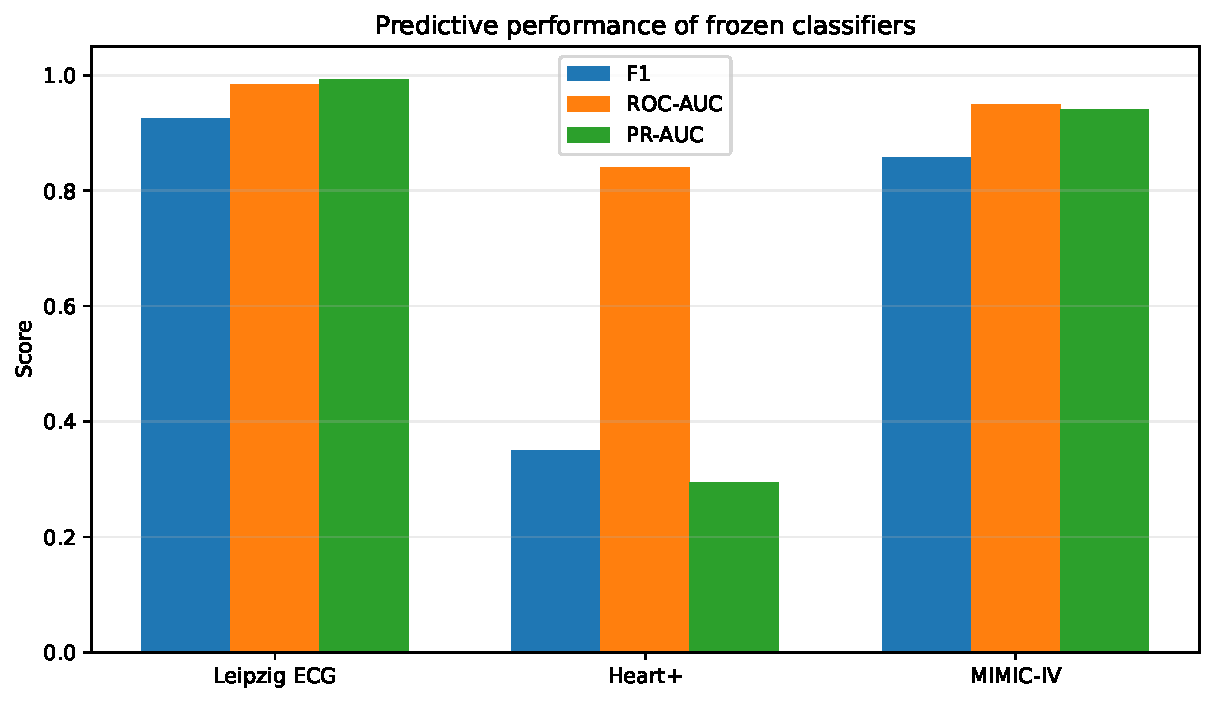
\includegraphics[width=0.82\linewidth]{figures/fig_classifier_performance.pdf}
    \caption{Predictive performance of the frozen polynomial classifiers on the
    outer test partitions. Heart+ has substantially lower F1 and PR-AUC, while
    Leipzig ECG and MIMIC-IV provide stronger discrimination.}
    \label{fig:classifier_performance}
\end{figure}

Leipzig ECG provides the strongest overall discrimination, with F1 of 0.9249
and ROC-AUC of 0.9833. MIMIC-IV also performs strongly, with F1 of 0.8574 and
ROC-AUC of 0.9496. Heart+ is considerably more difficult. Although its accuracy
is 0.8771, precision is only 0.2748, F1 is 0.3490, and PR-AUC is 0.2943.
This pattern is consistent with the strong class imbalance and shows why
accuracy alone is insufficient for interpreting Heart+.

The classifiers are used as fixed decision functions rather than as claims of
state-of-the-art predictive performance. The following counterfactual results
therefore describe recourse with respect to these frozen predictors and should
not be interpreted as causal effects on the underlying clinical outcomes.

\subsection{Counterfactual Quality and Robustness}
\label{subsec:cfe_baselines}

We first examine PrivDiCE at the primary privacy setting,
$\epsilon\approx4$. Table~\ref{tab:primary_directional} keeps the two
counterfactual directions separate. Here, $1\rightarrow0$ denotes movement
from the positive or adverse predicted class to the negative class, while
$0\rightarrow1$ denotes the reverse direction.

\begin{table}[!ht]
\centering
\caption{Directional performance of PrivDiCE at the primary privacy setting.}
\label{tab:primary_directional}
\resizebox{\linewidth}{!}{
\begin{tabular}{llccccccc}
\toprule
\textbf{Dataset}
& \textbf{Direction}
& \textbf{Yield@10 $\uparrow$}
& \textbf{Coverage@1 $\uparrow$}
& \textbf{Full-10 $\uparrow$}
& \textbf{Robust Yield@10 $\uparrow$}
& \textbf{Proximity $\downarrow$}
& \textbf{Sparsity $\uparrow$}
& \textbf{Diversity $\uparrow$} \\
\midrule
Leipzig ECG & $1\rightarrow0$
& 1.0000 & 1.0000 & 1.0000 & 0.8330 & 0.0724 & 0.7761 & 0.0677 \\
Leipzig ECG & $0\rightarrow1$
& 1.0000 & 1.0000 & 1.0000 & 0.7360 & 0.0673 & 0.7608 & 0.0740 \\
Heart+ & $1\rightarrow0$
& 0.9070 & 0.9400 & 0.8800 & 0.8720 & 0.0988 & 0.6472 & 0.0730 \\
Heart+ & $0\rightarrow1$
& 0.5460 & 0.7000 & 0.4700 & 0.5170 & 0.0928 & 0.6390 & 0.0478 \\
MIMIC-IV & $1\rightarrow0$
& 1.0000 & 1.0000 & 1.0000 & 0.8920 & 0.1175 & 0.5062 & 0.0918 \\
MIMIC-IV & $0\rightarrow1$
& 0.9900 & 0.9900 & 0.9900 & 0.9540 & 0.0885 & 0.6203 & 0.0740 \\
\bottomrule
\end{tabular}}
\end{table}

\begin{figure}[!ht]
    \centering
    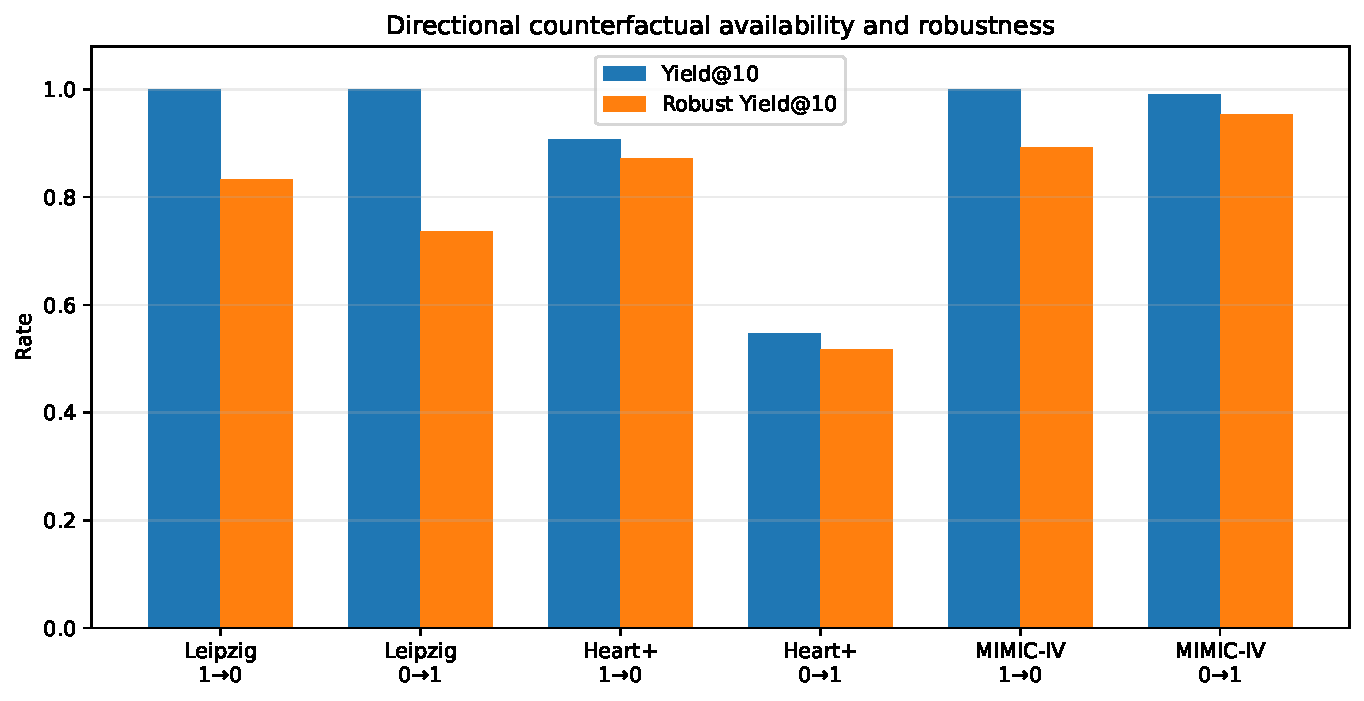
\includegraphics[width=\linewidth]{figures/fig_directional_yield_robustness.pdf}
    \caption{Directional counterfactual availability and robustness at
    $\epsilon\approx4$. Reporting both directions exposes the marked asymmetry
    of Heart+ that would be obscured by a single macro average.}
    \label{fig:directional_results}
\end{figure}

On Leipzig ECG, the operating budget is sufficient to fill all ten
counterfactual slots in both directions. The more informative differences are
therefore structural. Relative to iterative CounterGAN, PrivDiCE increases
sparsity from 0.1762 and 0.1663 to 0.7761 and 0.7608, respectively, while
reducing proximity from 0.1040 and 0.1181 to 0.0724 and 0.0673. This gain in
concision is accompanied by lower robust yield: 0.8330 and 0.7360 for
PrivDiCE compared with 0.9290 and 0.9930 for iterative CounterGAN. Sparse
search therefore improves the compactness of the explanations but does not
dominate robustness.

Heart+ presents the clearest directional asymmetry. PrivDiCE obtains Yield@10
of 0.9070 for $1\rightarrow0$, but only 0.5460 for $0\rightarrow1$.
Coverage decreases from 0.9400 to 0.7000 in the same comparison. Nevertheless,
relative to iterative CounterGAN, sparsity increases from 0.2960 and 0.3684 to
0.6472 and 0.6390, while proximity decreases from 0.1758 and 0.1442 to
0.0988 and 0.0928. Thus, the difficult reverse direction reflects reduced
counterfactual availability rather than a general loss of actionability among
the explanations that are found.

MIMIC-IV maintains high counterfactual availability in both directions.
Yield@10 is 1.0000 for $1\rightarrow0$ and 0.9900 for $0\rightarrow1$.
Compared with iterative CounterGAN, PrivDiCE substantially increases sparsity
and diversity, but robust yield decreases from 0.9640 and 0.9890 to 0.8920
and 0.9540. The plausibility distance also increases for the
$1\rightarrow0$ direction. These results again indicate a tradeoff among
sparsity, robustness, and data support.

Figure~\ref{fig:proximity_sparsity} provides a complementary view of the
actionability profile at the primary privacy setting.

\begin{figure}[!ht]
    \centering
    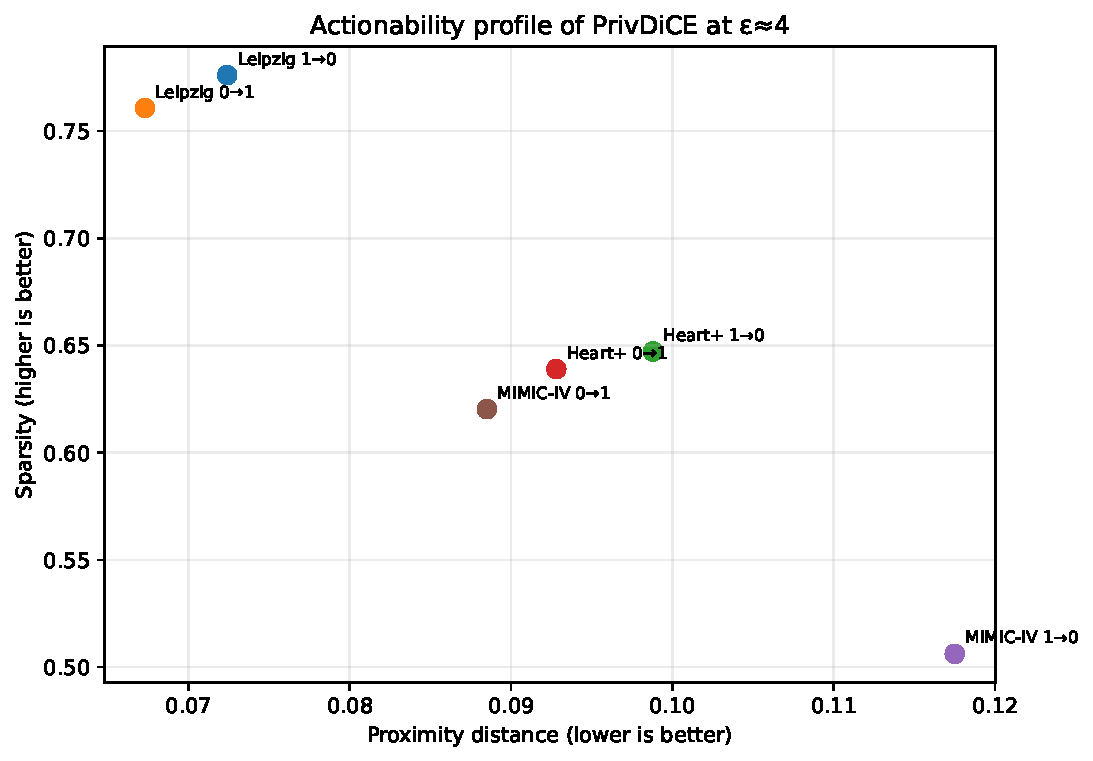
\includegraphics[width=0.80\linewidth]{figures/fig_proximity_sparsity.pdf}
    \caption{Proximity and sparsity of the primary PrivDiCE explanations.
    Lower proximity and higher sparsity correspond to smaller and more concise
    modifications.}
    \label{fig:proximity_sparsity}
\end{figure}

\subsection{Comparison with Counterfactual Baselines}
\label{subsec:macro_baselines}

Table~\ref{tab:cfe_macro_comparison} summarizes the main forward-evaluation
methods using equal-direction macro averages. Each direction receives weight
0.5. The macro table is intended as a compact summary and does not replace the
directional analysis above.

\begin{table}[!ht]
\centering
\caption{Equal-direction macro comparison at the operating candidate budget.
Values are from the fixed outer counterfactual run.}
\label{tab:cfe_macro_comparison}
\resizebox{\linewidth}{!}{
\begin{tabular}{llccccc}
\toprule
\textbf{Dataset}
& \textbf{Method}
& \textbf{Yield@10 $\uparrow$}
& \textbf{Robust Yield@10 $\uparrow$}
& \textbf{Proximity $\downarrow$}
& \textbf{Sparsity $\uparrow$}
& \textbf{Diversity $\uparrow$} \\
\midrule
\multirow{5}{*}{Leipzig ECG}
& Uniform Random       & 1.0000 & 0.8360 & 0.0932 & 0.2108 & 0.1205 \\
& Genetic CFE          & 1.0000 & 0.9010 & 0.0745 & 0.4148 & 0.0806 \\
& CounterGAN iterative & 1.0000 & 0.9610 & 0.1110 & 0.1713 & 0.0446 \\
& CounterGAN-SD non-DP & 1.0000 & 0.8160 & 0.0704 & 0.7735 & 0.0689 \\
& \textbf{PrivDiCE}    & 1.0000 & 0.7845 & 0.0698 & 0.7684 & 0.0709 \\
\midrule
\multirow{5}{*}{Heart+}
& Uniform Random       & 0.4650 & 0.4435 & 0.0672 & 0.5725 & 0.0513 \\
& Genetic CFE          & 0.3975 & 0.3650 & 0.0524 & 0.6539 & 0.0287 \\
& CounterGAN iterative & 0.7605 & 0.7540 & 0.1600 & 0.3322 & 0.0442 \\
& CounterGAN-SD non-DP & 0.7875 & 0.7585 & 0.1048 & 0.6240 & 0.0660 \\
& \textbf{PrivDiCE}    & 0.7265 & 0.6945 & 0.0958 & 0.6431 & 0.0604 \\
\midrule
\multirow{5}{*}{MIMIC-IV}
& Uniform Random       & 0.8410 & 0.6980 & 0.1121 & 0.1473 & 0.1327 \\
& Genetic CFE          & 0.9430 & 0.8445 & 0.0870 & 0.2726 & 0.0869 \\
& CounterGAN iterative & 0.9950 & 0.9765 & 0.1367 & 0.1238 & 0.0376 \\
& CounterGAN-SD non-DP & 0.9950 & 0.9185 & 0.1040 & 0.5418 & 0.0893 \\
& \textbf{PrivDiCE}    & 0.9950 & 0.9230 & 0.1030 & 0.5632 & 0.0829 \\
\bottomrule
\end{tabular}}
\end{table}

No method dominates all objectives. Leipzig ECG is saturated with respect to
Yield@10, yet the methods differ strongly in sparsity and robustness. PrivDiCE
and its non-private sparse counterpart produce substantially more concise
explanations than iterative CounterGAN, while the latter retains greater
robustness.

On Heart+, the non-private CounterGAN-SD configuration has the highest macro
Yield@10 among the listed forward-evaluation methods, whereas PrivDiCE retains
a similar sparse solution structure under differential privacy. The reduction
from 0.7875 to 0.7265 indicates a measurable utility cost at the primary DP
checkpoint. On MIMIC-IV, PrivDiCE and the non-private sparse configuration both
reach macro Yield@10 of 0.9950, while iterative CounterGAN again provides the
strongest robustness.

\subsection{Comparison with Official DiCE Implementations}
\label{subsec:official_dice_results}

The counted-budget benchmark is complemented by the official
\texttt{dice-ml} random and genetic implementations. These experiments use the
same outer factuals, desired labels, $K=10$, target margin, and domain
constraints. Their native stopping controls cannot be converted directly into
the counted candidate budget $B$, so this comparison evaluates matched
outcomes and constraints rather than equal computational access.

On Heart+, official DiCE Random obtains Yield@10 of 0.2440 for
$1\rightarrow0$ and 0.1710 for $0\rightarrow1$. Official DiCE Genetic reaches
the 20-second timeout for all evaluated Heart+ factuals under the specified
native configuration. This result characterizes the evaluated implementation
and timeout policy and is not evidence that genetic counterfactual search fails
in general.

MIMIC-IV illustrates why the two directions must remain separate. Official
DiCE Genetic reaches Yield@10 of 0.0250 for $1\rightarrow0$ but 0.9750 for
$0\rightarrow1$. In the latter direction, its robust yield is 0.9720, slightly
above PrivDiCE at 0.9540. PrivDiCE, however, has Full-10 of 0.9900 rather than
0.8600, sparsity of 0.6203 rather than 0.0395, and proximity of 0.0885 rather
than 0.2768. This comparison again reflects a multi-objective tradeoff rather
than a uniform ranking.

\subsection{Paired Statistical Comparisons}
\label{subsec:statistical_results}

Paired bootstrap intervals and Wilcoxon tests with Holm correction are used to
quantify factual-level differences between the primary PrivDiCE configuration
and selected comparators. Table~\ref{tab:paired_yield} reports representative
Yield@10 comparisons.

\begin{table}[!ht]
\centering
\caption{Selected paired factual-level comparisons for Yield@10. The reported
difference is PrivDiCE minus comparator.}
\label{tab:paired_yield}
\resizebox{\linewidth}{!}{
\begin{tabular}{llccc}
\toprule
\textbf{Dataset} & \textbf{Comparator}
& \textbf{Mean $\Delta$}
& \textbf{Bootstrap 95\% CI}
& \textbf{Holm $p$} \\
\midrule
Heart+ & DiCE-style gradient & 0.4690 & [0.4259, 0.5150] & $1.36\times10^{-24}$ \\
Heart+ & Genetic CFE         & 0.3290 & [0.2753, 0.3755] & $5.65\times10^{-18}$ \\
MIMIC-IV & DiCE-style gradient & 0.9105 & [0.8985, 0.9200] & $6.07\times10^{-37}$ \\
MIMIC-IV & Uniform Random      & 0.1540 & [0.1090, 0.1961] & $6.06\times10^{-6}$ \\
MIMIC-IV & Genetic CFE         & 0.0520 & [0.0260, 0.0745] & 0.0558 \\
MIMIC-IV & Wachter-style       & 0.9110 & [0.8990, 0.9200] & $4.71\times10^{-37}$ \\
\bottomrule
\end{tabular}}
\end{table}

The large differences against the gradient and Wachter-style baselines on
Heart+ and MIMIC-IV remain significant after Holm correction. The MIMIC-IV
comparison against Genetic CFE requires more caution. Its bootstrap interval
for the mean difference excludes zero, but the Holm-adjusted $p$-value is
0.0558. We therefore do not claim a statistically significant Yield@10
advantage over Genetic CFE after the applied multiple-comparison correction.

These tests quantify uncertainty across paired factual instances within the
fixed training run. They do not estimate stability across independent
CounterGAN retraining runs.

\subsection{Differential Privacy and Counterfactual Utility}
\label{subsec:privacy_utility}

The privacy sweep does not produce a monotonic change in every explanation
metric. Heart+ provides the clearest example because the reverse direction
remains difficult throughout the sweep.

\begin{figure}[!ht]
    \centering
    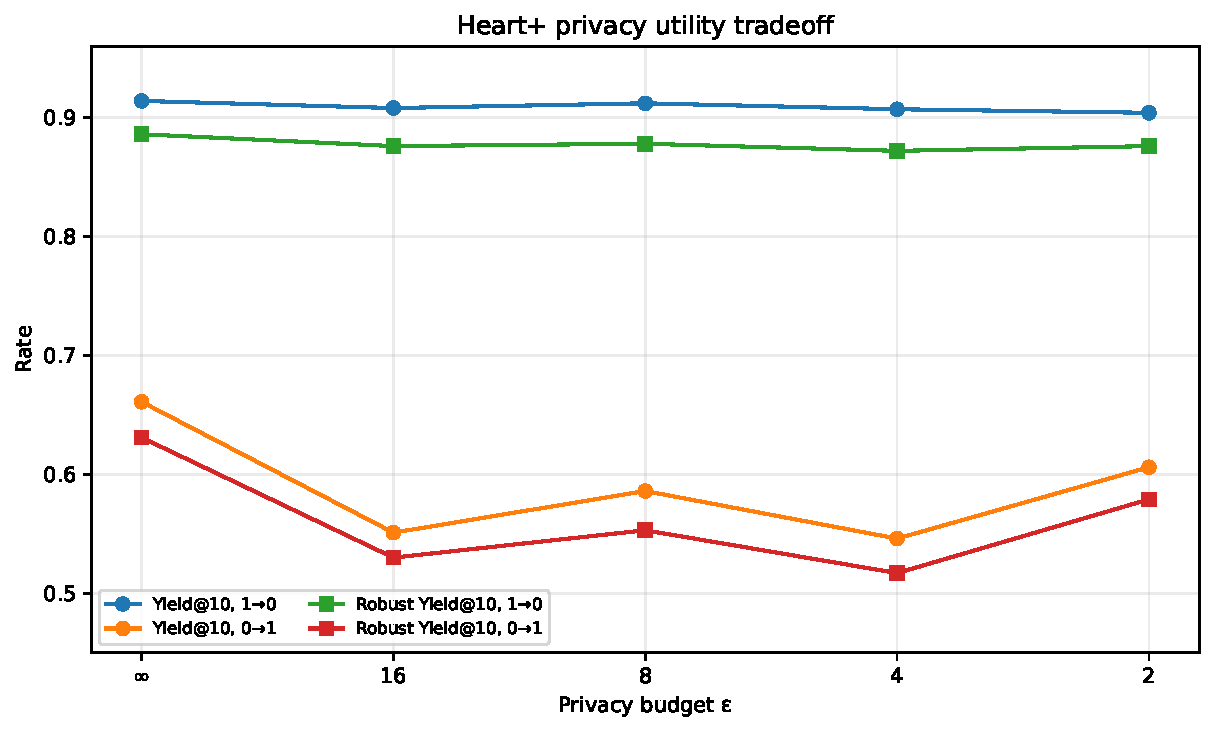
\includegraphics[width=0.88\linewidth]{figures/fig_heartplus_privacy_utility.pdf}
    \caption{Directional Heart+ privacy utility tradeoff. The reverse
    $0\rightarrow1$ direction remains substantially more difficult across the
    evaluated privacy budgets.}
    \label{fig:heartplus_privacy_utility}
\end{figure}

For $0\rightarrow1$, the non-private CounterGAN-SD configuration obtains
Yield@10 of 0.6610, compared with 0.5510, 0.5860, 0.5460, and 0.6060 for
$\epsilon\in\{16,8,4,2\}$, respectively. The primary $\epsilon\approx4$
checkpoint therefore incurs a visible loss in counterfactual availability in
this direction. The same change is not uniform across proximity, sparsity, or
robustness, so the privacy effect is better characterized as a
multidimensional tradeoff than as a single monotonic degradation curve.

The role of search budget is also particularly visible on Heart+. Figure
~\ref{fig:heartplus_budget} shows how additional candidate evaluations increase
the opportunity to fill the counterfactual archive.

\begin{figure}[!ht]
    \centering
    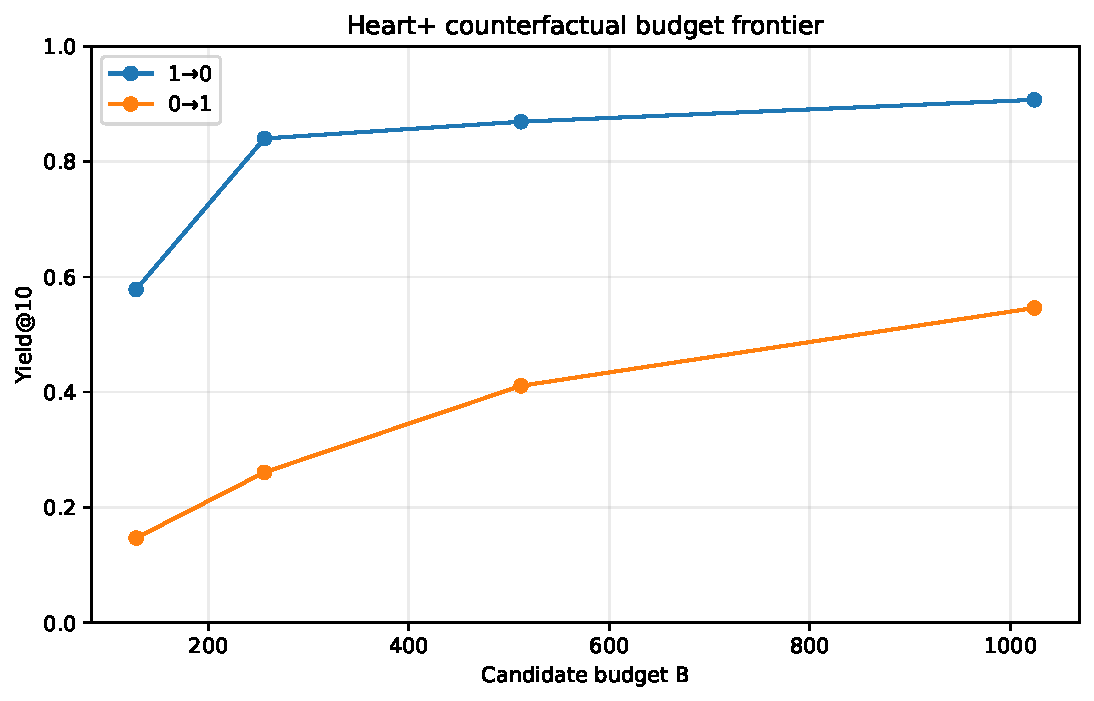
\includegraphics[width=0.82\linewidth]{figures/fig_heartplus_budget_frontier.pdf}
    \caption{Heart+ budget frontier for the primary PrivDiCE configuration.
    Increasing the candidate budget improves Yield@10 in both directions but
    also increases search effort.}
    \label{fig:heartplus_budget}
\end{figure}

As $B$ increases from 128 to 1024, Yield@10 rises from 0.5780 to 0.9070 for
$1\rightarrow0$ and from 0.1470 to 0.5460 for $0\rightarrow1$. The operating
budget was fixed using the inner protocol rather than selected from these outer
results.

\subsection{Empirical Privacy Leakage}
\label{subsec:privacy_attacks_results}

Formal differential privacy is complemented by empirical attacks that examine
different release surfaces. Table~\ref{tab:primary_privacy_results} summarizes
membership inference, exact and near duplication, and conditional attribute
inference at the primary privacy setting.

\begin{table}[!ht]
\centering
\caption{Selected empirical privacy results at $\epsilon\approx4$. Attribute
MAE is normalized and should be compared with the trivial baseline within the
same dataset.}
\label{tab:primary_privacy_results}
\resizebox{\linewidth}{!}{
\begin{tabular}{lccccc}
\toprule
\textbf{Dataset}
& \textbf{MIA AUC}
& \textbf{MIA 95\% CI}
& \textbf{Exact match}
& \textbf{Near duplicate}
& \textbf{Attribute MAE / trivial} \\
\midrule
Leipzig ECG & 0.5016 & [0.4935, 0.5095] & 0.0000 & 0.0000 & 0.0625 / 0.1022 \\
Heart+      & 0.4988 & [0.4914, 0.5062] & 0.0000 & 0.0404 & 0.4182 / 0.2500 \\
MIMIC-IV    & 0.5052 & [0.4985, 0.5123] & 0.0000 & 0.0000 & 0.0564 / 0.1093 \\
\bottomrule
\end{tabular}}
\end{table}

\begin{figure}[!ht]
    \centering
    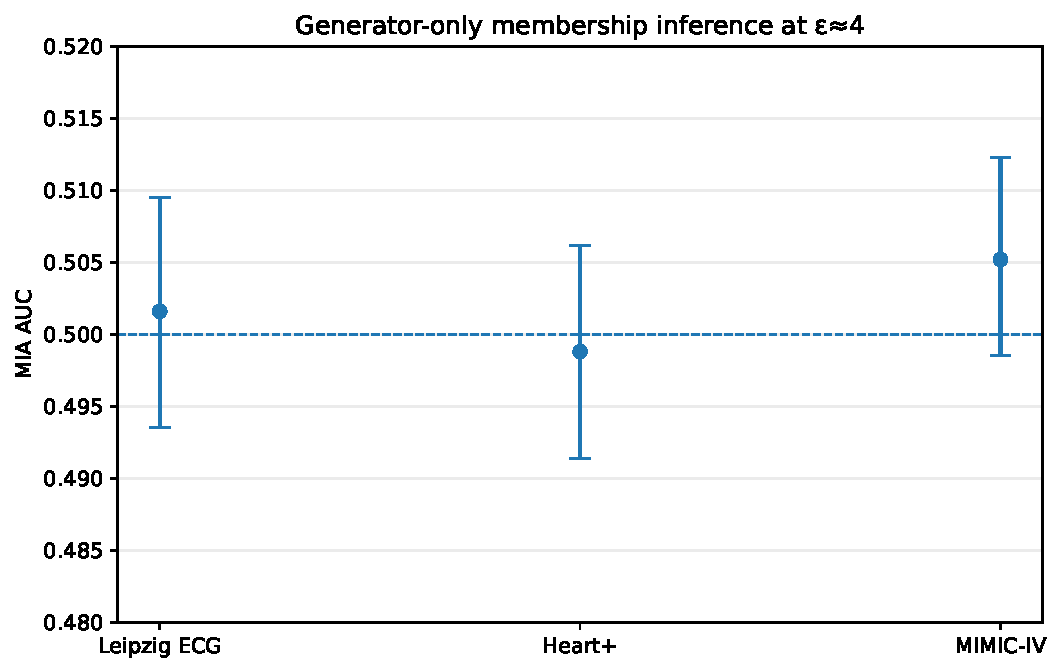
\includegraphics[width=0.76\linewidth]{figures/fig_mia_auc_ci.pdf}
    \caption{Strongest evaluated generator-only membership inference attack at
    the primary privacy setting. The dashed reference at AUC $=0.5$ denotes
    random discrimination. Error bars show the reported 95\% intervals across
    attack resampling.}
    \label{fig:mia_auc}
\end{figure}

At $\epsilon\approx4$, the strongest evaluated generator-only membership
attacks remain close to random discrimination. The AUC values are 0.5016 for
Leipzig ECG, 0.4988 for Heart+, and 0.5052 for MIMIC-IV. This result indicates
weak membership discrimination under the evaluated release surface, but it
does not establish that all privacy attacks fail. For example, the Leipzig ECG
$\epsilon=2$ checkpoint reaches MIA AUC of 0.6054, showing that empirical
attack behavior need not vary monotonically with the nominal privacy budget.

Exact record matches are zero at the primary setting for all three datasets.
Heart+, however, has a near-duplicate rate of 0.0404, so the memorization
results should not be summarized as showing an absence of approximate
memorization.

Conditional attribute inference provides another caution. For Leipzig ECG,
the normalized attack MAE is 0.0625 compared with a trivial baseline of 0.1022.
For MIMIC-IV the corresponding values are 0.0564 and 0.1093. In both cases the
attacker outperforms the trivial predictor under the implemented protocol.
Heart+ shows the opposite pattern, with attack MAE of 0.4182 compared with a
trivial baseline of 0.2500. These results describe release-level inference risk
and are distinct from the formal training-membership guarantee of DP-SGD.

Explanation linkage reveals an additional direction-dependent surface.
Figure~\ref{fig:mimic_linkage} summarizes the strongest directional warning on
MIMIC-IV.

\begin{figure}[!ht]
    \centering
    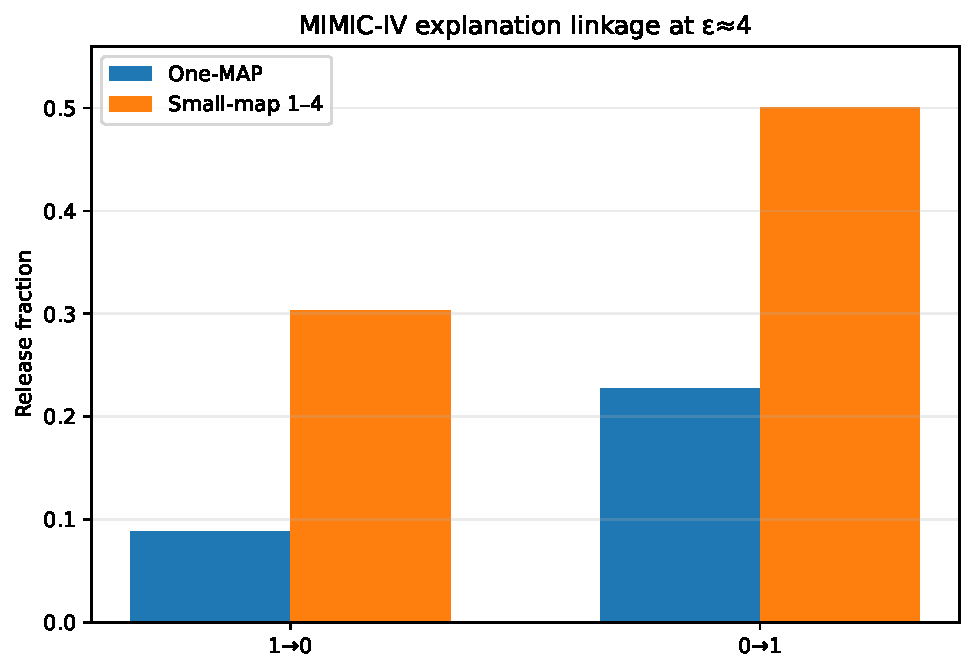
\includegraphics[width=0.72\linewidth]{figures/fig_mimic_linkage.pdf}
    \caption{Directional explanation-linkage exposure on MIMIC-IV at
    $\epsilon\approx4$. One-MAP is the fraction of released signatures that
    map to one auxiliary record, while Small-map measures mappings to one to
    four auxiliary records.}
    \label{fig:mimic_linkage}
\end{figure}

For MIMIC-IV, One-MAP increases from 0.0880 in the $1\rightarrow0$ direction
to 0.2273 in the reverse direction, while Small-map increases from 0.3030 to
0.5010. Similar directional behavior appears for several alternative methods,
suggesting that the leakage is influenced by the release signature and
auxiliary population rather than by the DP checkpoint alone. This result
demonstrates why membership inference should not be used as the sole empirical
privacy indicator.

\subsection{CKKS Correctness and System Cost}
\label{subsec:he_efficiency_results}

Encrypted candidate evaluation is implemented using real TenSEAL CKKS
ciphertexts. Table~\ref{tab:he_efficiency} reports the selected population
sizes and the measured execution cost.

\begin{table}[!ht]
\centering
\caption{CKKS execution at the selected operating population.}
\label{tab:he_efficiency}
\resizebox{\linewidth}{!}{
\begin{tabular}{lrrrrrr}
\toprule
\textbf{Dataset}
& $\boldsymbol{P}$
& $\boldsymbol{N}$
& \textbf{Total latency (s)}
& \textbf{Upload (MB)}
& \textbf{Download (MB)}
& \textbf{Label agreement} \\
\midrule
Leipzig ECG & 64  & 16,384 & 83.0892 & 26.9604 & 0.2469 & 1.0000 \\
Heart+      & 128 & 8,192  & 28.0602 & 10.7024 & 0.0886 & 1.0000 \\
MIMIC-IV    & 64  & 16,384 & 80.6351 & 48.9961 & 0.2357 & 1.0000 \\
\bottomrule
\end{tabular}}
\end{table}

CKKS preserves the plaintext classification label for all evaluated candidate
cohorts under the selected profiles. The observed agreement of 1.0000 is a
numerical correctness result for the tested encrypted execution and should not
be interpreted as evidence of counterfactual utility.

Figure~\ref{fig:he_latency_breakdown} shows where the system cost is incurred.

\begin{figure}[!ht]
    \centering
    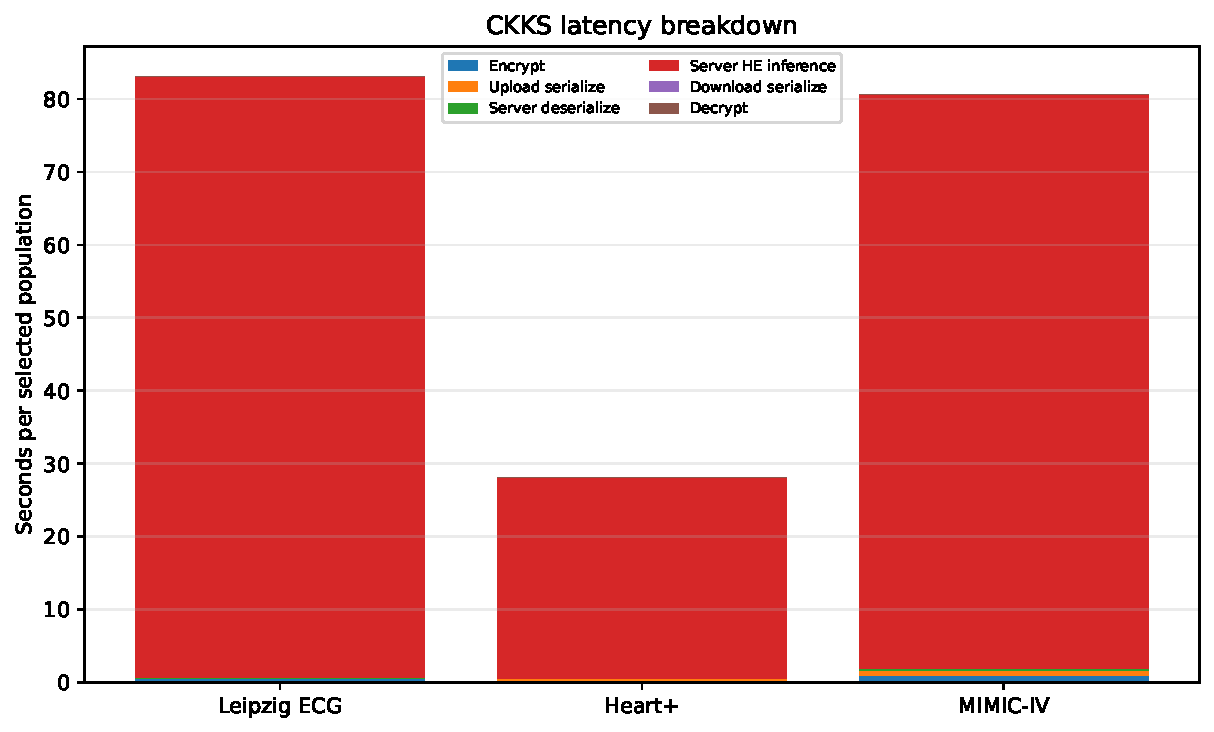
\includegraphics[width=0.88\linewidth]{figures/fig_he_latency_breakdown.pdf}
    \caption{Latency breakdown of CKKS candidate evaluation at the selected
    population sizes. Server-side homomorphic inference dominates the measured
    latency for all three datasets.}
    \label{fig:he_latency_breakdown}
\end{figure}

Server-side HE inference accounts for approximately 82.4327 seconds of the
83.0892-second Leipzig total, 27.4963 seconds of the 28.0602-second Heart+
total, and 78.7849 seconds of the 80.6351-second MIMIC-IV total. Encryption,
serialization, and decryption are comparatively small. MIMIC-IV has the
largest upload volume because the processed prediction model receives 40
encrypted input features.

A boundary-focused stress cohort also preserves label agreement of 1.0000 for
all three datasets. The maximum observed logit errors are
$6.27\times10^{-6}$ for Leipzig ECG, $0.0034$ for Heart+, and
$7.73\times10^{-5}$ for MIMIC-IV, while the closest evaluated plaintext logits
remain approximately 0.10 from the decision boundary. These findings explain
the observed agreement for the tested cohorts but do not establish a guarantee
for arbitrary ciphertext inputs.

The measured CKKS benchmark represents encrypted model evaluation for packed
candidate populations. It is not a direct full-cohort measurement of the
complete iterative counterfactual search. When search rounds are combined with
the measured per-round CKKS cost, the resulting quantity is an estimated
composed system cost rather than a directly observed end-to-end encrypted run.

\subsection{Qualitative Inspection}
\label{subsec:qualitative_results}

The quantitative evaluation is complemented by representative counterfactual
inspection. Ten factual instances are selected for each dataset, with five
from each prediction direction. The cases correspond to predefined
predicted-probability quantiles from 0.1 to 0.9 rather than manually selected
successful examples. Failed cases are retained as \texttt{NO VALID CFE} in the
qualitative artifact. This protocol reduces selective presentation and provides
a direct check of the raw-domain changes after inverse transformation.

\subsection{Cross-Dataset Findings}
\label{subsec:cross_dataset_synthesis}

The results provide a consistent but non-uniform picture across the three
datasets. First, the frozen polynomial classifiers provide sufficient
predictive discrimination for the counterfactual study, although Heart+ remains
challenging because of its class imbalance. Second, PrivDiCE produces highly
sparse counterfactuals while retaining high availability on Leipzig ECG and
MIMIC-IV, whereas the reverse Heart+ direction remains substantially harder.

Third, semantic sparse and diverse search introduces measurable tradeoffs.
Explanations become more concise than those produced by iterative CounterGAN,
but robustness can decrease. Differential privacy introduces an additional
utility cost in difficult regions rather than causing a uniform change in all
metrics.

Fourth, empirical privacy conclusions depend on the attack surface. Membership
inference is close to random at the primary operating point, yet near-duplicate,
attribute-inference, and explanation-linkage analyses reveal residual exposure
that is not captured by membership AUC alone.

Finally, CKKS reproduces the plaintext labels on the evaluated candidate
cohorts, demonstrating that encrypted model evaluation can be integrated with
the counterfactual workflow. Its main limitation is computational cost, with
homomorphic model evaluation dominating the measured latency. Overall, the
experiments support the feasibility of jointly addressing counterfactual
actionability, training-data privacy, and inference confidentiality, while also
showing that these objectives remain subject to utility, robustness, privacy,
and systems tradeoffs.



\section{Discussion and Implications}
\label{sec:discussion}

The experimental results show that privacy-preserving counterfactual
explanation cannot be characterized by a single measure of validity, privacy,
or computational performance. PrivDiCE combines three components that address
different requirements: a differentially private generator, semantic sparse
and diverse search, and CKKS-protected model evaluation. The results indicate
that these components can operate within a common framework, but they also
introduce distinct tradeoffs that become visible across datasets,
counterfactual directions, and privacy settings.

\subsection{Actionability Requires More Than Counterfactual Validity}
\label{subsec:discussion_actionability}

A central observation from the experiments is that high counterfactual validity
does not necessarily imply high explanation quality. This is particularly clear
on Leipzig ECG, where several methods achieve complete Yield@10 and Coverage@1
at the operating budget. Once validity is saturated, the main differences
between methods appear in proximity, sparsity, diversity, and robustness.

PrivDiCE substantially increases sparsity relative to iterative CounterGAN while
also reducing the magnitude of the required changes. This behavior reflects the
combined effect of feature and group sparsification, semantic restoration, and
diversity-aware archive selection. The resulting explanations are therefore
more concise in the processed feature space and generally require fewer
unnecessary modifications.

However, the same results also show that sparsification should not be treated
as an objective that can be improved without consequence. On Leipzig ECG and
MIMIC-IV, PrivDiCE produces considerably sparser explanations than iterative
CounterGAN, but robust yield is lower. Removing apparently unnecessary feature
changes can reduce the distance by which a counterfactual crosses the local
decision region, making the resulting explanation more sensitive to small
feasible perturbations. This explains why explanation concision and robustness
can move in opposite directions.

The comparison therefore supports a multi-objective interpretation of
counterfactual quality. A method that produces highly sparse explanations is
not necessarily preferable if those explanations are unstable, while a robust
counterfactual may require changes to more features than a user would consider
practical. The appropriate operating point depends on the intended use of the
explanation and should be evaluated across these dimensions rather than by
validity alone.


\subsection{Directional Asymmetry Is an Important Property of Recourse}
\label{subsec:discussion_directionality}

The bidirectional evaluation reveals that counterfactual difficulty can depend
strongly on the requested prediction direction. Heart+ provides the clearest
example. At the primary privacy setting, Yield@10 is 0.9070 for
$1\rightarrow0$ but only 0.5460 for $0\rightarrow1$, with corresponding
Coverage@1 values of 0.9400 and 0.7000. The same asymmetry appears across
several baseline methods.

This result indicates that counterfactual generation should not be summarized
only by a pooled or macro average. A high aggregate score can conceal a
direction for which recourse is substantially more difficult. In imbalanced
datasets, the geometry of the learned decision function and the density of the
target region may differ substantially between directions. Counterfactual
search must therefore solve two different problems rather than a symmetric
label-flipping task.

The Heart+ results also illustrate why candidate budget is an important part of
the evaluation protocol. Increasing the candidate budget improves
counterfactual availability in both directions, but the difficult
$0\rightarrow1$ direction remains substantially below the reverse direction.
Additional search therefore reduces, but does not remove, directional
difficulty.

These observations motivate reporting counterfactual results separately by
direction whenever the application admits semantically distinct transitions.
The equal-direction macro values used in this work are intended only as compact
summaries and should not replace directional analysis.


\subsection{Differential Privacy Introduces a Nonuniform Utility Tradeoff}
\label{subsec:discussion_dp}

Differential privacy is used in PrivDiCE to limit the influence of individual
training records on the released generative component. The privacy sweep shows
that the resulting utility cost is neither uniform nor monotonic across
counterfactual metrics.

On Leipzig ECG and MIMIC-IV, counterfactual availability remains high across
the primary operating configurations. In contrast, Heart+ exhibits a clearer
utility loss. In the difficult $0\rightarrow1$ direction, the non-private
CounterGAN-SD configuration achieves Yield@10 of 0.6610, whereas the primary
DP configuration reaches 0.5460. This difference provides direct evidence that
privacy can reduce the ability of the generator and subsequent search to find a
sufficient number of valid explanations in difficult regions.

At the same time, smaller values of $\epsilon$ do not consistently produce
lower utility across all metrics. DP-SGD modifies the learned generator through
gradient clipping and stochastic noise, and the resulting candidate
distribution can interact with the geometry of the frozen predictor in
nonlinear ways. Consequently, a single trained checkpoint may improve one
metric while degrading another even under a stronger nominal privacy setting.

For this reason, the privacy sweep should not be interpreted as a deterministic
ordering in which utility decreases monotonically with $\epsilon$. The formal
privacy parameter controls the training guarantee, whereas observed
counterfactual utility depends on the learned generator, search procedure, and
target decision region. The primary operating point should therefore be viewed
as a selected compromise rather than an intrinsically optimal privacy level.


\subsection{Formal Privacy and Empirical Leakage Measure Different Risks}
\label{subsec:discussion_privacy}

The empirical privacy results reinforce the distinction between a formal
differential privacy guarantee and observed leakage from released explanations,
consistent with recent counterfactual-specific privacy studies
\cite{ezzeddine2026privatecf,babaei2026privacycf}.
At the primary privacy setting, the strongest generator-only membership
inference attacks remain close to random discrimination on all three datasets.
This provides encouraging evidence for the evaluated membership surface, but it
does not imply that the released generator or its explanations are free from
other forms of information leakage.

The memorization analysis illustrates this distinction. Exact training-record
matches are absent at the primary privacy setting, yet Heart+ retains a
nonzero near-duplicate rate. Exact-match statistics alone would therefore give
an incomplete picture of memorization behavior.

Conditional attribute inference provides another example. On Leipzig ECG and
MIMIC-IV, the evaluated attacker achieves lower normalized reconstruction error
than the corresponding trivial baseline. Thus, useful information about the
selected attribute remains inferable under the evaluated release protocol even
though membership inference is close to random. Heart+ exhibits the opposite
pattern for the selected attribute, showing that empirical leakage also depends
on the dataset and target attribute.

Explanation linkage exposes a further release-level risk. On MIMIC-IV, the
$0\rightarrow1$ direction produces considerably higher One-MAP and Small-map
rates than the reverse direction. Importantly, similar directional behavior is
also observed for alternative counterfactual methods. The linkage risk is
therefore influenced not only by generator training but also by the structure
of the released counterfactuals and the auxiliary population available to an
attacker.

These findings support evaluating privacy through multiple complementary
surfaces. Differential privacy provides a formal guarantee for the training
mechanism, while membership inference, memorization, attribute inference, and
explanation linkage examine different empirical consequences of releasing a
generator or explanation. None of these empirical attacks alone is a complete
privacy measure, and their results should not be interpreted as replacing the
formal DP guarantee.


\subsection{Homomorphic Encryption Protects Evaluation but Not the Entire
Explanation Pipeline}
\label{subsec:discussion_he}

The CKKS experiments demonstrate that remote prediction can be performed over
encrypted counterfactual populations while preserving the decisions of the
plaintext prediction graph on the evaluated cohorts. Label agreement reaches
1.0000 under the selected cryptographic profiles for all three datasets, and
the boundary-focused stress tests remain consistent with plaintext inference.

This agreement is important because counterfactual validity depends directly on
the prediction oracle. A small numerical discrepancy is acceptable only if it
does not change the classification or invalidate the required target margin.
The observed CKKS approximation errors remain below the distance of the tested
boundary cases from the decision threshold, explaining the complete agreement
in the evaluated cohorts.

Nevertheless, encrypted evaluation remains the dominant systems cost.
Server-side CKKS model evaluation accounts for most of the measured latency,
particularly for Leipzig ECG and MIMIC-IV. The cost depends on the polynomial
network, modulus chain, input dimensionality, and packing configuration rather
than on counterfactual generation alone. MIMIC-IV also incurs the largest
communication volume because its processed representation requires more feature
ciphertexts.

Population packing partially mitigates this cost by allowing several candidate
values to occupy different CKKS slots and be processed in parallel. As
population size increases, the encrypted latency per round remains relatively
stable while the cost per candidate decreases. This behavior makes population
evaluation particularly suitable for counterfactual search, where many
candidate solutions must be scored against the same model.

It is important, however, to distinguish encrypted model evaluation from a
fully encrypted counterfactual pipeline. In PrivDiCE, candidate generation,
semantic projection, sparse refinement, archive management, and final
explanation selection remain on the client side. CKKS protects the
privacy-sensitive interaction with the remote prediction model. The framework
should therefore be described as counterfactual generation with encrypted model
evaluation rather than end-to-end homomorphic counterfactual generation.


\subsection{Implications for Privacy-Preserving Explainable Systems}
\label{subsec:discussion_implications}

The results suggest several broader implications for the design of
privacy-preserving explanation systems.

First, different privacy mechanisms should be associated with the specific
information surface they protect. Differential privacy limits dependence on
individual training records but does not conceal a new client's factual record
from a prediction service. Homomorphic encryption protects the query during
remote computation but does not control information contained in the released
explanation. Combining the two mechanisms is therefore meaningful because they
address different stages of the explanation lifecycle.

Second, explanation utility should be evaluated jointly with the failure rate.
Metrics such as proximity, sparsity, plausibility, and diversity are typically
defined only when a valid counterfactual exists. A method that returns very few
counterfactuals may consequently appear strong on conditional quality metrics.
The Yield@10 and Coverage@1 definitions used in this study retain failed queries
in the evaluation and reduce this source of optimistic reporting.

Third, actionability should be enforced during generation and search rather than
added only after explanations have been selected. PrivDiCE projects candidates
onto the feasible domain and restores semantic groups before final selection.
This design avoids presenting explanations that score well numerically but
violate immutable attributes or categorical structure.

Finally, the results show that privacy, actionability, robustness, and
cryptographic efficiency cannot be optimized independently. Greater
sparsification can reduce robustness, stronger privacy can reduce
counterfactual availability, and encrypted deployment can introduce substantial
latency. A practical deployment therefore requires an operating point selected
according to the application's relative tolerance for these competing costs.


\subsection{Limitations}
\label{subsec:limitations}

Several limitations should be considered when interpreting the results.

The first limitation concerns training variability. The primary plaintext
counterfactual experiments use one generator training seed for each
configuration. The paired bootstrap intervals and Wilcoxon tests quantify
variation across factual instances conditional on the trained checkpoint, but
they do not establish stability across independent generator retraining runs.
Additional multi-seed retraining would provide stronger evidence regarding the
variance introduced by private generative training.

Second, the three datasets do not provide identical levels of subject
independence. Leipzig ECG uses a subject-disjoint split, and Heart+ keeps exact
feature groups disjoint across partitions. The derived MIMIC-IV cohort supplied to the experimental pipeline does not
retain a patient identifier, so the experiment relies on a stratified row
split. Results on MIMIC-IV should therefore not be interpreted
as patient-level generalization.

Third, counterfactual explanations describe changes with respect to the learned
prediction function. They do not establish that modifying the corresponding
clinical attributes would cause the predicted health outcome to change in the
real world. The explanations should therefore be interpreted as model-based
recourse rather than causal treatment recommendations.

Fourth, the empirical privacy attacks represent specific attacker models and
auxiliary information. A weak result for one attack does not establish
resistance to stronger or differently informed adversaries. In particular, the
observed linkage and attribute-inference results show that residual release
risks can remain even when membership inference is close to random.

Fifth, the threat model for encrypted inference is honest but curious. The
server is assumed to execute the prescribed CKKS computation correctly.
Protection against malicious model servers, malformed ciphertext processing,
or verifiable execution would require additional cryptographic mechanisms and
is outside the scope of the present framework.

Finally, the reported composed HE search cost is obtained by combining measured
per-round CKKS execution with the observed number of search rounds. It is not a
direct measurement of the complete counterfactual workflow running over
ciphertexts for every outer factual instance. A production-scale evaluation of
the complete client-server deployment would therefore be a useful extension of
this study.

\section{Conclusion}
\label{sec:conclusion}

This work presented PrivDiCE, a privacy-preserving framework for
actionable counterfactual explanation that combines differential privacy,
semantic sparse and diverse counterfactual search, and CKKS-protected model
evaluation. The framework separates two complementary privacy surfaces:
differential privacy limits the influence of individual training records on the
released generative component, while homomorphic encryption protects sensitive
client records and candidate counterfactuals during remote model evaluation.
This separation allows privacy protection to be incorporated directly into the
counterfactual workflow without requiring the complete explanation procedure to
be executed under encryption.

Experiments on Leipzig ECG, Heart+, and MIMIC-IV show that PrivDiCE can produce
concise and feasible counterfactual explanations while preserving high
counterfactual availability in several settings. The results also demonstrate
that explanation quality is inherently multi-objective. Increased sparsity and
smaller modifications can be accompanied by reduced robustness, while the
effect of differential privacy varies across datasets and prediction
directions. Heart+ in particular reveals a pronounced directional asymmetry and
a clearer privacy--utility tradeoff, illustrating the importance of evaluating
counterfactual recourse separately in each prediction direction.

The privacy analysis further shows that no single empirical attack is sufficient
to characterize the privacy of released explanations. Membership inference is
close to random discrimination at the primary privacy operating point, whereas
memorization, conditional attribute inference, and explanation-linkage analyses
identify residual risks that depend on the dataset and release direction. These
findings reinforce the distinction between the formal training guarantee
provided by differential privacy and empirical leakage that may arise from the
released counterfactuals themselves.

The CKKS evaluation demonstrates that encrypted model inference can reproduce
the corresponding plaintext decisions on the evaluated candidate cohorts while
preventing the remote prediction server from observing plaintext candidate
values. The main practical limitation remains computational cost, with
homomorphic model evaluation accounting for most of the measured execution
time. Population packing mitigates this overhead by evaluating multiple
counterfactual candidates in parallel, but further optimization is required for
latency-sensitive deployment.

Overall, PrivDiCE demonstrates that actionable counterfactual explanation,
training-data privacy, and confidential remote prediction can be integrated
within a common framework. At the same time, the results show that privacy,
actionability, robustness, and computational efficiency cannot be optimized independently. Future work will therefore focus on improving the robustness of sparse counterfactuals, reducing encrypted inference cost, extending the threat
model to malicious servers, evaluating additional empirical privacy attacks,
and examining variability across multiple independent private-generator
training runs.

\section*{Acknowledgements}

The authors acknowledge the institutional support of the Academy of
Cryptography Techniques, Hanoi University of Science and Technology, Hanoi
University of Civil Engineering, and the Japan Advanced Institute of Science
and Technology.

\section*{CRediT authorship contribution statement}

\noindent
\textbf{Viet-Nhat Nguyen:}
Conceptualization, Methodology, Software, Investigation, Data curation,
Validation, Visualization.

\noindent
\textbf{Anh-Tu Tran:}
Conceptualization, Methodology, Formal analysis, Validation,
Writing -- original draft, Visualization.

\noindent
\textbf{The-Dung Luong:}
Conceptualization, Methodology, Validation, Writing -- review \& editing,
Supervision.

\noindent
\textbf{Van-Nam Huynh:}
Conceptualization, Methodology, Supervision, Project administration, Funding
acquisition, Writing -- review \& editing.

\section*{Data Availability}

The Leipzig ECG cohort is derived from the Leipzig Heart Center ECG-Database
released through PhysioNet
\cite{PhysioNet-leipzig-heart-center-ecg-1.0.0}. The MIMIC-IV cohort is
derived from the PhysioNet MIMIC-IV release
\cite{PhysioNet-mimiciv-2.2,johnson2023mimiciv} and remains subject to the
access conditions of the source resource. Heart+ is the merged heart-risk
cohort used by the experimental pipeline. To ensure that this derived cohort
can be identified unambiguously, the reproducibility materials specify its
source manifest, file checksum, cleaning rules, and split manifest. The
preprocessing configuration, cohort-selection rules, and random seeds required
to regenerate the reported experimental partitions are included with the
reproducibility materials.

\section*{Code Availability}

The implementation comprises the polynomial prediction models, conditional
CounterGAN training, DP-SGD, semantic projection, feature and group
sparsification, budgeted candidate refinement, MMR archive selection, empirical
privacy attacks, and TenSEAL CKKS candidate evaluation. The supporting
configuration records dependency versions, privacy-accounting settings, CKKS
parameter profiles, random seeds, and scripts used to regenerate the reported
tables and figures. Code, experiment configurations, aggregate result tables,
and redistributable artifacts are available in the public reproducibility
repository accompanying this article.
Access-controlled MIMIC-IV inputs and row-level derivatives are not redistributed
and remain subject to the PhysioNet data-use agreement.

\section*{Ethical Statement}

This study uses benchmark or secondary clinical datasets and does not involve
direct interaction with human participants. PrivDiCE is intended as a
privacy-preserving explanation framework for predictive models. Its
counterfactual outputs describe model-based recourse and should not be
interpreted as autonomous clinical decisions, causal treatment effects, or
medical recommendations.

\section*{Declaration of competing interest}

The authors declare that they have no known competing financial interests or
personal relationships that could have appeared to influence the work reported
in this paper.

\bibliography{ref}{}

\end{document}
